%=======================================================================
%  Global Air Connectivity and Trade Openness, 1996-2023
%  Target: Transportation Research Part A: Policy and Practice (Elsevier)
%  SELF-CONTAINED: bibliography embedded via filecontents; all tables inline.
%  Upload this .tex plus the figures:
%     GACI_base_map.png  GACI_continent_trend.png  GACI_contrib_trade_3panel.png
%     GACI_covid_shock_3panel.png  GACI_hetero_quartile.png
%     GACI_method_construction.png  GACI_rank_bump.png  GACI_rf_quintile.png
%  Compile: pdflatex -> bibtex -> pdflatex x2
%  Rev 2026-09-02: authoryear (TRA Harvard) citations, DOI links, larger captions, 1996-2023 unified, Fig.2 re-rendered
%=======================================================================
\begin{filecontents*}[overwrite]{GACI_TRA_refs.bib}
@article{Cristea_2011, title={Buyer-seller relationships in international trade: Evidence from {U.S.} states' exports and business-class travel}, volume={84}, DOI={10.1016/j.jinteco.2011.02.003}, number={2}, journal={J. Int. Econ.}, author={Cristea, Anca D.}, year={2011}, pages={207--220} }
@article{Hovhannisyan_2015, title={International business travel: an engine of innovation?}, volume={20}, DOI={10.1007/s10887-014-9107-7}, number={1}, journal={J. Econ. Growth}, author={Hovhannisyan, Nune and Keller, Wolfgang}, year={2015}, pages={75--104} }
@article{Belenkiy_2012, title={Face-to-Face Exports: The Role of Business Travel in Trade Promotion}, volume={51}, DOI={10.1177/0047287512437857}, number={5}, journal={J. Travel Res.}, author={Belenkiy, Maksim and Riker, David}, year={2012}, pages={632--639} }
@techreport{Startz_2016, title={The Value of Face-to-Face: Search and Contracting Problems in {Nigerian} Trade}, author={Startz, Meredith}, year={2018}, type={SSRN Working Paper}, number={3096685}, institution={Social Science Research Network}, DOI={10.2139/ssrn.3096685} }
@article{Campante_2017, title={Long-Range Growth: Economic Development in the Global Network of Air Links}, volume={133}, DOI={10.1093/qje/qjx050}, number={3}, journal={Q. J. Econ.}, author={Campante, Filipe and Yanagizawa-Drott, David}, year={2018}, pages={1395--1458} }
@article{Brueckner_2003, title={Airline Traffic and Urban Economic Development}, volume={40}, DOI={10.1080/0042098032000094388}, number={8}, journal={Urban Stud.}, author={Brueckner, Jan K.}, year={2003}, pages={1455--1469} }
@article{Rauch_1999, title={Networks versus markets in international trade}, volume={48}, DOI={10.1016/s0022-1996(98)00009-9}, number={1}, journal={J. Int. Econ.}, author={Rauch, James E.}, year={1999}, pages={7--35} }
@article{Allen_2014, title={Information Frictions in Trade}, volume={82}, DOI={10.3982/ecta10984}, number={6}, journal={Econometrica}, author={Allen, Treb}, year={2014}, pages={2041--2083} }
@article{Hummels_2007, title={Transportation Costs and International Trade in the Second Era of Globalization}, volume={21}, DOI={10.1257/jep.21.3.131}, number={3}, journal={J. Econ. Perspect.}, author={Hummels, David}, year={2007}, pages={131--154} }
@article{Hummels_2013, title={Time as a Trade Barrier}, volume={103}, DOI={10.1257/aer.103.7.2935}, number={7}, journal={Am. Econ. Rev.}, author={Hummels, David L. and Schaur, Georg}, year={2013}, pages={2935--2959} }
@article{Frankel_1999, title={Does Trade Cause Growth?}, volume={89}, DOI={10.1257/aer.89.3.379}, number={3}, journal={Am. Econ. Rev.}, author={Frankel, Jeffrey A. and Romer, David}, year={1999}, pages={379--399} }
@article{Feyrer_2019, title={Trade and Income---{Exploiting} Time Series in Geography}, volume={11}, DOI={10.1257/app.20170616}, number={4}, journal={Am. Econ. J. Appl. Econ.}, author={Feyrer, James}, year={2019}, pages={1--35} }
@article{Alcala_2004, title={Trade and Productivity}, volume={119}, DOI={10.1162/0033553041382139}, number={2}, journal={Q. J. Econ.}, author={Alcal\'a, Francisco and Ciccone, Antonio}, year={2004}, pages={613--646} }
@article{Redding_2004, title={Economic geography and international inequality}, volume={62}, DOI={10.1016/j.jinteco.2003.07.001}, number={1}, journal={J. Int. Econ.}, author={Redding, Stephen and Venables, Anthony J.}, year={2004}, pages={53--82} }
@article{Donaldson_2018, title={Railroads of the {Raj}: Estimating the Impact of Transportation Infrastructure}, volume={108}, DOI={10.1257/aer.20101199}, number={4-5}, journal={Am. Econ. Rev.}, author={Donaldson, Dave}, year={2018}, pages={899--934} }
@article{Donaldson_2016, title={Railroads and {American} Economic Growth: A Market Access Approach}, volume={131}, DOI={10.1093/qje/qjw002}, number={2}, journal={Q. J. Econ.}, author={Donaldson, Dave and Hornbeck, Richard}, year={2016}, pages={799--858} }
@article{Pascali_2017, title={The Wind of Change: Maritime Technology, Trade, and Economic Development}, volume={107}, DOI={10.1257/aer.20140832}, number={9}, journal={Am. Econ. Rev.}, author={Pascali, Luigi}, year={2017}, pages={2821--2854} }
@article{GoldsmithPinkham_2020, title={{Bartik} Instruments: What, When, Why, and How}, volume={110}, DOI={10.1257/aer.20181047}, number={8}, journal={Am. Econ. Rev.}, author={Goldsmith-Pinkham, Paul and Sorkin, Isaac and Swift, Henry}, year={2020}, pages={2586--2624} }
@article{Borusyak_2022, title={Quasi-Experimental Shift-Share Research Designs}, volume={89}, DOI={10.1093/restud/rdab030}, number={1}, journal={Rev. Econ. Stud.}, author={Borusyak, Kirill and Hull, Peter and Jaravel, Xavier}, year={2022}, pages={181--213} }
@article{Adao_2019, title={Shift-Share Designs: Theory and Inference}, volume={134}, DOI={10.1093/qje/qjz025}, number={4}, journal={Q. J. Econ.}, author={Ad\~ao, Rodrigo and Koles\'ar, Michal and Morales, Eduardo}, year={2019}, pages={1949--2010} }
@article{Conley_2012, title={Plausibly Exogenous}, volume={94}, DOI={10.1162/REST_a_00139}, number={1}, journal={Rev. Econ. Stat.}, author={Conley, Timothy G. and Hansen, Christian B. and Rossi, Peter E.}, year={2012}, pages={260--272} }
@article{Cheung_2020, title={The evolution of aviation network: {Global Airport Connectivity Index} 2006--2016}, volume={133}, DOI={10.1016/j.tre.2019.101826}, journal={Transp. Res. Part E Logist. Transp. Rev.}, author={Cheung, Tommy K.Y. and Wong, Collin W.H. and Zhang, Anming}, year={2020}, pages={101826} }
@techreport{Bertoli_2016, title={The {CERDI}-seadistance database}, institution={CERDI}, number={2016/7}, author={Bertoli, Simone and Goujon, Micha\"el and Santoni, Olivier}, year={2016} }
@techreport{Gaulier_2010, title={{BACI}: International Trade Database at the Product-Level. {The} 1994--2007 Version}, institution={CEPII}, type={CEPII Working Paper}, number={2010-23}, DOI={10.2139/ssrn.1994500}, author={Gaulier, Guillaume and Zignago, Soledad}, year={2010} }
@techreport{Arezki_2009, title={Tourism Specialization and Economic Development: Evidence from the {UNESCO} {World Heritage List}}, institution={International Monetary Fund}, type={IMF Working Paper}, number={09/176}, DOI={10.5089/9781451873238.001}, author={Arezki, Rabah and Cherif, Reda and Piotrowski, John}, year={2009} }
@article{Faber_2019, title={Tourism and Economic Development: Evidence from {Mexico}'s Coastline}, volume={109}, DOI={10.1257/aer.20161434}, number={6}, journal={Am. Econ. Rev.}, author={Faber, Benjamin and Gaubert, Cecile}, year={2019}, pages={2245--2293} }
@article{Copeland_1991, title={Tourism, Welfare and De-industrialization in a Small Open Economy}, volume={58}, DOI={10.2307/2554696}, number={232}, journal={Economica}, author={Copeland, Brian R.}, year={1991}, pages={515--529} }
@article{Holzner_2011, title={Tourism and economic development: The beach disease?}, volume={32}, DOI={10.1016/j.tourman.2010.08.007}, number={4}, journal={Tour. Manag.}, author={Holzner, Mario}, year={2011}, pages={922--933} }
@article{Bertacchini_2016, title={The politicization of {UNESCO} {World Heritage} decision making}, volume={167}, DOI={10.1007/s11127-016-0332-9}, number={1-2}, journal={Public Choice}, author={Bertacchini, Enrico and Liuzza, Claudia and Meskell, Lynn and Saccone, Donatella}, year={2016}, pages={95--129} }
@techreport{UNCTAD_2021, title={{Review of Maritime Transport 2021}}, institution={United Nations Conference on Trade and Development}, author={{UNCTAD}}, year={2021}, address={Geneva} }
@misc{IATA_cargo, title={The Value of Air Cargo}, howpublished={International Air Transport Association, \url{https://www.iata.org/en/programs/cargo/sustainability/benefits/}}, author={{IATA}}, year={2026}, note={Accessed 2 July 2026} }
@article{Adler_2014, title={Air transport liberalization and airport slot allocation: The case of the {Northeast Asian} transport market}, volume={62}, DOI={10.1016/j.tra.2014.02.003}, journal={Transp. Res. Part A Policy Pract.}, author={Adler, Nicole and Fu, Xiaowen and Oum, Tae Hoon and Yu, Chunyan}, year={2014}, pages={3--19} }
@article{Amico_2026, title={Air connectivity boosts urban attractiveness for global firms}, volume={3}, DOI={10.1038/s44284-025-00361-4}, number={1}, journal={Nat. Cities}, author={Amico, Ambra and Duarte, Fabio and Liao, Wen-Chi and Zheng, Siqi}, year={2026}, pages={78--88} }
@article{Antras_2013, title={Organizing the global value chain}, volume={81}, DOI={10.3982/ECTA10813}, number={6}, journal={Econometrica}, author={Antr\`as, Pol and Chor, Davin}, year={2013}, pages={2127--2204} }
@article{Burghouwt_2013, title={Connectivity in air transport networks: An assessment of models and applications}, volume={47}, DOI={10.3828/jtep.2013.47.1.35}, number={1}, journal={J. Transp. Econ. Policy}, author={Burghouwt, Guillaume and Redondi, Renato}, year={2013}, pages={35--53} }
@article{Burghouwt_2015, title={In the wake of liberalisation: Long-term developments in the {EU} air transport market}, volume={43}, DOI={10.1016/j.tranpol.2015.05.006}, journal={Transp. Policy}, author={Burghouwt, Guillaume and de Wit, Jaap G.}, year={2015}, pages={104--113} }
@article{Gillen_2002, title={Measuring the economic effects of bilateral liberalization air transport}, volume={38}, DOI={10.1016/S1366-5545(02)00003-0}, number={3-4}, journal={Transp. Res. Part E Logist. Transp. Rev.}, author={Gillen, David and Harris, Richard and Oum, Tae Hoon}, year={2002}, pages={155--174} }
@article{Henderson_2002, title={Global production networks and the analysis of economic development}, volume={9}, DOI={10.1080/09692290210150842}, number={3}, journal={Rev. Int. Polit. Econ.}, author={Henderson, Jeffrey and Dicken, Peter and Hess, Martin and Coe, Neil and Yeung, Henry Wai-Chung}, year={2002}, pages={436--464} }
@article{Jiang_2026, title={Innovation on wings: The impact of air route opening on cross-city collaborative innovation}, volume={103}, DOI={10.1016/j.asieco.2026.102140}, journal={J. Asian Econ.}, author={Jiang, Weijie and Fang, Yuqian}, year={2026}, pages={102140} }
@article{Johnson_2017, title={A portrait of trade in value-added over four decades}, volume={99}, DOI={10.1162/REST_a_00665}, number={5}, journal={Rev. Econ. Stat.}, author={Johnson, Robert C. and Noguera, Guillermo}, year={2017}, pages={896--911} }
@article{Lenaerts_2021, title={The economic impact of aviation: A review on the role of market access}, volume={91}, DOI={10.1016/j.jairtraman.2020.102000}, journal={J. Air Transp. Manag.}, author={Lenaerts, Bert and Allroggen, Florian and Malina, Robert}, year={2021}, pages={102000} }
@article{Liao_2026, title={Uneven skies: Long-term global inventory and equity analysis of aviation emissions}, volume={154}, DOI={10.1016/j.trd.2026.105286}, journal={Transp. Res. Part D Transp. Environ.}, author={Liao, Weijun and Yue, Shuai and Wang, Xiaoqian and Cao, Fangyu and Ji, Qing and Wang, Chunan and Fan, Ying}, year={2026}, pages={105286} }
@article{OKelly_2026, title={Worldwide airline network evolution between 2000 and 2023: A systematic analysis of hubs, hub links, allocations, and direct links}, volume={203}, DOI={10.1016/j.tra.2025.104744}, journal={Transp. Res. Part A Policy Pract.}, author={O'Kelly, Morton and Sun, Xiaoqian and Wandelt, Sebastian}, year={2026}, pages={104744} }
@article{Oum_2024, title={Impact of air connectivity on bilateral service export and import trade: The case of {China}}, volume={148}, DOI={10.1016/j.tranpol.2024.01.015}, journal={Transp. Policy}, author={Oum, Tae Hoon and Wu, Xiangru and Wang, Kun}, year={2024}, pages={219--233} }
@article{Sun_2021, title={{COVID-19} pandemic and air transportation: Successfully navigating the paper hurricane}, volume={94}, DOI={10.1016/j.jairtraman.2021.102062}, journal={J. Air Transp. Manag.}, author={Sun, Xiaoqian and Wandelt, Sebastian and Zheng, Changhong and Zhang, Anming}, year={2021}, pages={102062} }
@article{Sun_2024, title={On the relationship between air connectivity and economic development: A comparative analysis of inequality evolution for 2000--2019}, volume={2}, DOI={10.1016/j.team.2024.09.006}, journal={Transp. Econ. Manag.}, author={Sun, Xiaoqian and Wandelt, Sebastian and Zhang, Anming}, year={2024}, pages={310--321} }
@article{Wandelt_2025, title={Network structures in air transportation: A comprehensive review of applications and challenges}, volume={126}, DOI={10.1016/j.jairtraman.2025.102794}, journal={J. Air Transp. Manag.}, author={Wandelt, Sebastian and Wang, Shuang and Chen, Xinyue and Zheng, Changhong and Chang, Shuming and Sun, Xiaoqian}, year={2025}, pages={102794} }
@article{Zhang_2026, title={Beyond direct flights: Higher-order connectivity in {China}'s international air cargo network}, volume={209}, DOI={10.1016/j.tra.2026.105013}, journal={Transp. Res. Part A Policy Pract.}, author={Zhang, Linfeng and Yang, Hangjun and Bian, Lei and Zhang, Junjie}, year={2026}, pages={105013} }
@article{Zheng_2020, title={Comparison of the spaces of call and traffic flows: An empirical study of {Qianzhong} urban region, {China}}, volume={107}, DOI={10.1016/j.cities.2020.102927}, journal={Cities}, author={Zheng, Longfei and Long, Fenjie and Zhang, Su}, year={2020}, pages={102927} }
@article{Zhou_2021, title={Vulnerability of the worldwide air transportation network to global catastrophes such as {COVID-19}}, volume={154}, DOI={10.1016/j.tre.2021.102469}, journal={Transp. Res. Part E Logist. Transp. Rev.}, author={Zhou, Yaoming and Kundu, Tanmoy and Qin, Wei and Goh, Mark and Sheu, Jiuh-Biing}, year={2021}, pages={102469} }
@article{Soderlund_2023, title={The importance of business travel for trade: Evidence from the liberalization of the {Soviet} airspace}, volume={145}, DOI={10.1016/j.jinteco.2023.103812}, journal={J. Int. Econ.}, author={S\"oderlund, Bengt}, year={2023}, pages={103812} }
@article{Harrigan_2010, title={Airplanes and comparative advantage}, volume={82}, DOI={10.1016/j.jinteco.2010.07.002}, number={2}, journal={J. Int. Econ.}, author={Harrigan, James}, year={2010}, pages={181--194} }
@article{Hummels_2010, title={Hedging price volatility using fast transport}, volume={82}, DOI={10.1016/j.jinteco.2010.05.002}, number={1}, journal={J. Int. Econ.}, author={Hummels, David L. and Schaur, Georg}, year={2010}, pages={15--25} }
@article{Blonigen_2015, title={Air service and urban growth: Evidence from a quasi-natural policy experiment}, volume={86}, DOI={10.1016/j.jue.2015.02.001}, journal={J. Urban Econ.}, author={Blonigen, Bruce A. and Cristea, Anca D.}, year={2015}, pages={128--146} }
@article{Umana_2019, title={Do visas hinder international trade in goods?}, volume={140}, DOI={10.1016/j.jdeveco.2019.05.002}, journal={J. Dev. Econ.}, author={Umana-Dajud, Camilo}, year={2019}, pages={106--126} }
@article{Fageda_2017, title={International air travel and FDI flows: Evidence from {Barcelona}}, volume={57}, DOI={10.1111/jors.12325}, number={5}, journal={J. Reg. Sci.}, author={Fageda, Xavier}, year={2017}, pages={858--883} }
@article{Alderighi_2017, title={Fly and trade: Evidence from the {Italian} manufacturing industry}, volume={9}, DOI={10.1016/j.ecotra.2017.02.001}, journal={Econ. Transp.}, author={Alderighi, Marco and Gaggero, Alberto A.}, year={2017}, pages={51--60} }
@article{Micco_2006, title={Competition regimes and air transport costs: The effects of open skies agreements}, volume={70}, DOI={10.1016/j.jinteco.2005.06.015}, number={1}, journal={J. Int. Econ.}, author={Micco, Alejandro and Serebrisky, Tom\'as}, year={2006}, pages={25--51} }
@article{Yilmazkuday_2017, title={The role of direct flights in trade costs}, volume={153}, DOI={10.1007/s10290-016-0263-z}, number={2}, journal={Rev. World Econ.}, author={Yilmazkuday, Demet and Yilmazkuday, Hakan}, year={2017}, pages={249--270} }
\end{filecontents*}

\documentclass[review,3p,times,authoryear]{elsarticle}

\usepackage{lineno,hyperref}
\usepackage{amsmath,amssymb}
\usepackage{graphicx}
\usepackage{booktabs}
\usepackage{threeparttable}
\usepackage{multirow}
\usepackage{url}
\usepackage{float}

% --- Reference-list formatting (TRA / Elsevier Harvard): DOIs as https://doi.org/... links,
%     no "doi:" / "URL:" prefixes, URLs in text font (Guide for Authors sample style).
\urlstyle{same}
\providecommand{\DOIprefix}{}\renewcommand{\DOIprefix}{}
\providecommand{\URLprefix}{}\renewcommand{\URLprefix}{}
\providecommand{\doi}[1]{}\renewcommand{\doi}[1]{\href{https://doi.org/#1}{\nolinkurl{https://doi.org/#1}}}

% --- Figure/table captions: elsarticle sets captions in \footnotesize; use \small with a bold label.
\makeatletter
\long\def\@makecaption#1#2{%
  \vskip\abovecaptionskip\small
  \sbox\@tempboxa{\textbf{#1.} #2}%
  \ifdim \wd\@tempboxa >\hsize
    \textbf{#1.} #2\par
  \else
    \global \@minipagefalse
    \hb@xt@\hsize{\hfil\box\@tempboxa\hfil}%
  \fi
  \vskip\belowcaptionskip}
\makeatother
\journal{Transportation Research Part A: Policy and Practice}

\newcommand{\sym}[1]{\ensuremath{^{#1}}}

\begin{document}

\begin{frontmatter}

\title{Global Air Connectivity and Trade Openness, 1996--2023}

\author[a]{[Author]\corref{cor1}}
\ead{[email]}
\cortext[cor1]{Corresponding author.}
\author[a]{[Co-author]}
\address[a]{[Affiliation]}

\begin{abstract}
We estimate the causal effect of global air connectivity on merchandise (goods) trade using a panel of 184 countries over 1996--2023. Air connectivity is measured by the Global Air Connectivity Index (GACI), a
network-centrality summary of each country's position in the world airport network. To address the endogenous expansion of air routes, we exploit exogenous variation in connectivity using an instrumental variable based on time-invariant natural heritage endowments interacted with global tourism cycles. Two-stage least squares (2SLS) with country and year fixed effects yields a goods-trade-volume elasticity of $2.30$, which decomposes exactly into a trade-openness elasticity of $1.30$ and a GDP-scale elasticity of $1.00$. The estimates are robust across alternative instruments, an alternative connectivity measure, and falsification checks. Product-level trade data reveal the mechanism: connectivity shifts the trade mix toward high value-to-weight goods and, more tentatively, intermediate goods, the margins on which air transport operates, and this compositional shift absorbs the openness effect entirely once controlled for. Returns are highly uneven: the openness payoff to connectivity declines with both baseline income and baseline connectivity, so the marginal value of an additional air link is largest in poorer and under-connected economies and smaller in well-connected advanced hubs. A counterfactual analysis suggests that improvements in global air connectivity since 1996 contributed substantially to the expansion of world merchandise trade. The results identify airport and route investment and air-service liberalisation as concrete, spillover-aware levers for trade integration.
\end{abstract}

\begin{keyword}
Air connectivity \sep international trade \sep shift-share instrument \sep
network centrality \sep trade composition \sep global value chains
\end{keyword}

\end{frontmatter}

\linenumbers

%=======================================================================
\section{Introduction}
%=======================================================================
What does air connectivity do, economically? At its core it shrinks economic distance: a country's position in the world air network determines how near it is, in time and cost, to the markets, suppliers, and partners that make up the global economy. Connectivity is therefore a form of accessibility, and the economic content of accessibility is the capacity to exchange. Among the flows that distance impedes (people, capital, ideas, goods), the one that responds most robustly, and that we can observe most cleanly, is trade: that trade declines with distance is among the most durable regularities in economics \citep{Redding_2004,Hummels_2007}. If air links pull a country closer to the rest of the world, trade is where that proximity should appear first and most sharply.

Yet the consequences of improved air connectivity have not been clearly established. We are motivated by two research questions. First, we ask whether a country's position in the global air network causally raises
its trade, and if so, on which margin the effect operates: the openness of the economy or its overall scale, and through which kinds of goods. This question matters for policy because governments invest heavily in
airports, hub development, and air-service liberalisation, and the justification for these investments depends on whether connectivity deepens integration rather than merely accompanying income growth. We examine trade because it is among the most direct measures of a country's integration into the world economy, and greater trade openness is associated with higher productivity and income \citep{Frankel_1999,Alcala_2004,Feyrer_2019}. Second, we ask who gains and when: whether the trade response differs across richer and poorer, better- and less-connected economies, and whether the relationship is symmetric when connectivity collapses rather than expands. This question matters because, if the effect is concentrated in poorer and less-connected economies, connectivity is directly relevant for
development policy. It also matters because aviation networks, unlike most other transport infrastructure, can contract within months, so the consequences of such contractions are a policy concern in their own right.

A natural objection is that most trade does not travel by air: more than 80 per cent of international trade volume is carried by sea \citep{UNCTAD_2021}. The objection, however, concerns weight rather than value. Measured by value, the basis on which trade openness is defined, air cargo accounts for roughly one third of world trade \citep{IATA_cargo}, and our connectivity measure is built from passenger networks, which affect trade through channels that do not require aircraft to carry the goods at all. Air connectivity moves the people who make trade happen: buyers meeting sellers, managers inspecting suppliers, the face-to-face contact on which trade in differentiated goods depends \citep{Rauch_1999,Cristea_2011,Startz_2016}. It thus lowers the cost of the transaction whatever mode later moves the cargo. It moves the high-value,
time-sensitive slice of goods for which speed is worth the freight premium, largely in the belly holds of the same passenger aircraft, where each day in transit carries an ad-valorem cost of roughly 0.6--2.1\%
\citep{Hummels_2007,Hummels_2013}. And it underpins participation in global value chains, in which engineers, samples, and urgent components move by air while the resulting gross trade flows multiply across borders.
Each channel makes a testable prediction about what kind of trade should respond, and we test these predictions with product-level data below.

Trade also offers an identification advantage over broader economic outcomes such as GDP or income. These aggregates are the distant end of a long and confounded chain, whereas trade is the proximate, observable
margin on which connectivity acts, and the development literature locates the long-run income gains from integration on exactly this margin. A country's trade openness is, in effect, its degree of participation in the global division of labour, and air connectivity is one of the physical substrates of that participation. Asking
whether connectivity raises trade is thus asking the central question of transport economics: whether better physical access translates into deeper economic integration.

Our research questions require a connectivity measure that is continuous, comparable across countries, and available over a long period. Existing measures do not satisfy these requirements together: route-opening
indicators are binary and discard the intensive margin, bilateral frequencies do not capture indirect connections through third countries, and network-based indices are available only at the airport level and for
recent years. We therefore construct a country-level connectivity panel, the Global Air Connectivity Index (GACI). Applying the airport-level centrality methodology of \citet{Cheung_2020}, we rebuild the global air
network from annual airline schedules for each year from 1996 to 2023, covering between 3{,}171 and 3{,}833 active airports per year, and aggregate the airport-level scores into a country-year panel of 184
countries. To our knowledge, this is the longest country-level panel of air connectivity currently available. The sample period includes the liberalisation of the late 1990s, the expansion of Gulf and Asian hubs,
and the collapse and recovery associated with COVID-19. Because no single aggregate captures every dimension of a country's connectivity, we employ three measures: a capacity-weighted mean of airport-level GACI, which uses the entire airport system while placing most weight on the dominant hubs and serves as our headline measure of hub quality; the maximum across a country's airports; and their sum.

Examining the impact of air connectivity on trade requires attention to endogeneity concerns. Because a country's connectivity and its trade are jointly determined, ordinary least squares estimates are unlikely to carry a causal interpretation: airlines add routes and capacity where trade and income are already growing, and both connectivity and trade respond to common shocks. We therefore instrument connectivity with a shift-share design that interacts a predetermined national exposure with a global demand cycle. The exposure is a country's endowment of natural and mixed UNESCO World Heritage sites, an amenity rooted in geography and history rather than in economic activity; the shift is the global cycle in international tourist arrivals. When world tourism demand expands, airlines disproportionately add service to heritage-endowed countries, so the interaction isolates the component of network growth driven by leisure travel rather than by goods trade. Country fixed effects absorb the endowment itself and year fixed effects absorb the global cycle, so that identification rests only on their interaction; the outcome, goods trade, excludes tourism receipts by construction. Section~\ref{sec:strategy} formalises the design and \ref{sec:robust} examines the exclusion restriction directly.

This paper builds on, and departs from, three literatures. The first is the economics of air transport and development. \citet{Brueckner_2003} shows that airline traffic raises service employment in US metropolitan areas; \citet{Campante_2017} exploit a discontinuity in long-haul aircraft range to show that direct intercontinental links increase business connections and local economic activity; and \citet{Hovhannisyan_2015} document that inbound business travel raises innovation in destination industries. This work establishes that air links matter for economic outcomes, but its outcomes are local employment, firm linkages, and innovation rather than national trade, and its variation is route- or city-level rather than a country's overall position in the network. The second is the literature identifying trade-driven income gains from geography and historical
infrastructure. \citet{Frankel_1999} instrument openness with geographic trade shares; \citet{Feyrer_2019} uses the changing relative importance of air and sea distance to show that the gains from trade increasingly travel
through the air; \citet{Donaldson_2018} and \citet{Donaldson_2016} show that railroads raised incomes through market access in colonial India and the nineteenth-century United States; and \citet{Pascali_2017} shows that
the steamship distributed the gains from trade unevenly across countries. This literature treats transport as a deep determinant of trade-driven development, but its contemporary aviation counterpart is thin: the trade
margin on which a country's air-network position acts has not been isolated with a design that treats the network itself as endogenous. The third is the literature that links aviation directly to trade. Business travel
promotes exports in relationship-intensive sectors \citep{Cristea_2011,Startz_2016,Soderlund_2023}, consistent with the role of face-to-face contact in trade in differentiated goods \citep{Rauch_1999}, and the time costs of shipping give high value-to-weight goods a distinct air margin \citep{Hummels_2013}. This literature identifies the channels through which air links can create trade, but it typically works with bilateral route variation and stops short of asking whether a country's overall network position raises its total goods trade. 

Taken together, these studies leave open two questions: whether a country's overall position in the air network raises its total goods trade, and which trade responds. Addressing them, this paper makes two contributions. First, we provide causal estimates of the effect of connectivity on goods trade, decompose the effect into an openness margin and a scale margin, translate the estimates into aggregate magnitudes for world trade, and characterise how the response varies across countries, over time, and between expansions and contractions of the network. Second, using product-level trade data, we test the predictions of the channels described above: whether connectivity shifts the composition of trade toward high value-to-weight goods and intermediate inputs, and whether this compositional margin accounts for the aggregate effect. Methodologically, our instrument draws on the shift-share framework and its inference tools \citep{GoldsmithPinkham_2020,Adao_2019,Borusyak_2022}. Section~\ref{sec:literature} develops these literatures and the resulting hypotheses in detail.

The remainder of the paper proceeds as follows. Section~\ref{sec:literature} reviews the literature and develops the hypotheses. Section~\ref{sec:data} describes the construction of the GACI panel, the trade outcomes, and the instrument. Section~\ref{sec:strategy} presents the empirical strategy. Section~\ref{sec:results} reports the main results, including heterogeneity across countries and over time, the mechanism analysis, the aggregate contribution of connectivity growth, and connectivity-collapse episodes. Section~\ref{sec:discussion} discusses the findings and their limitations, and Section~\ref{sec:conclusion} concludes. 

%=======================================================================
\section{Literature review and hypothesis development}
\label{sec:literature}
% [Section 2 incorporated from "GACI and trade_Section 2_260814.docx".]
%=======================================================================
\subsection{Literature review}

The global aviation system has undergone a fundamental transformation over
the past several decades. It evolved from a sparse network of
intercontinental trunk routes into a dense, highly interconnected global
system. This transformation has been driven by sustained growth in passenger
demand, the expansion of international flight networks, and the increasing
integration of emerging economies into global mobility systems
\citep{Liao_2026,OKelly_2026}. During 1996--2023, the number of active
airports connected to the global aviation network increased from 3{,}171 to
3{,}833.\footnote{Data come from the Official Airline Guide (OAG) database.}
Alongside this physical expansion, aviation has become increasingly important
for global economic exchange. Although air transport accounts for only a
small share of international trade by volume, it represents approximately one
third of global trade value because air transportation is particularly suited
to high-value, time-sensitive, and technologically advanced goods
\citep{IATA_cargo}. Beyond transporting passengers and goods, aviation
networks reduce effective economic distance by connecting firms, markets, and
production locations across countries \citep{Lenaerts_2021}. As a result,
aviation connectivity has become a fundamental component of contemporary
globalisation and international economic integration \citep{Zhang_2026}.

The growing importance of aviation connectivity has generated substantial
policy interest among governments, airports, and airlines \citep{Adler_2014}.
Countries increasingly compete to develop global aviation hubs, strengthen
their positions within international networks, and attract economic
activities through airport investment and air-service liberalisation,
including open-skies agreements \citep{Gillen_2002,Burghouwt_2015}.
Long-range air links reshape global economic geography by integrating cities
into wider international networks, thereby accelerating growth in newly
connected locations \citep{Campante_2017}, and quasi-experimental evidence
from the 1978 United States airline deregulation shows that expanded air
traffic raises metropolitan population, income, and employment growth
\citep{Blonigen_2015}. However, aviation connectivity
differs from many conventional transportation infrastructures in an important
way: connectivity depends not only on physical infrastructure but also on the
operation of network links \citep{Wandelt_2025}. As a result, aviation
networks can expand rapidly but can also contract abruptly in response to
external shocks. The COVID-19 pandemic provided a striking example, as
international flight networks collapsed within months following travel
restrictions and demand shocks \citep{Sun_2021}. Unlike ports, highways, or
railways, whose physical capacity generally remains stable during
disruptions, aviation connectivity can deteriorate quickly because it is
sustained by dynamic interactions between airlines, airports, and passengers
\citep{Zhou_2021}.

A key challenge in studying aviation connectivity is how to quantify a
country's position within the global aviation network. Early studies
typically measured connectivity using simple indicators, such as the number
of routes, flight frequencies, or passenger volumes. Although informative,
these measures capture the scale of activity rather than the structural
position of locations within the network \citep{Burghouwt_2013}. Recent
research has therefore shifted toward network-based measures that incorporate
centrality, accessibility, and indirect connections \citep{Wandelt_2025}.
These measures reflect the idea that connectivity is fundamentally
relational, depending not only on the number of links but also on the
importance and reach of connected destinations \citep{Cheung_2020}.
Centrality-based measures better capture economic accessibility than
traditional bilateral distance measures, as they incorporate indirect
connections and network spillovers \citep{Zhou_2021}. In this paper, we
follow the literature \citep{Cheung_2020} by constructing a Global Air
Connectivity Index (GACI). This index summarises each country's position in
the global airport network by aggregating airport-level centrality measures
into a country-level indicator of accessibility.

The relevance of air connectivity for economic outcomes is closely tied to
its role in facilitating face-to-face communications and trade
\citep{Sun_2024}. Trade, including goods and services trade, is widely
recognised as the most direct and observable margin through which reductions
in economic distance translate into income gains. The gravity literature
provides robust evidence that trade flows decline strongly with geographic
distance and transport costs \citep{Redding_2004,Zheng_2020}, and the
literature on trade and growth establishes that greater trade openness is
associated with higher productivity and income levels \citep{Alcala_2004}.
More recent work highlights the dynamic evolution of transport costs in
shaping globalisation patterns \citep{Amico_2026}. For example,
\citet{Feyrer_2019} exploits the divergence between air and sea distances
over time and shows that the gains from trade increasingly operate through
air-based connections, underscoring the growing importance of fast transport
modes in global integration. Historical evidence further reinforces this
view: railroads played a central role in expanding market access and raising
local incomes \citep{Donaldson_2016,Donaldson_2018}, while maritime
technological change redistributed the gains from trade across countries in
uneven ways \citep{Pascali_2017}. These studies collectively highlight
transportation infrastructure as a fundamental determinant of trade-driven
development.

A relatively small but growing literature directly links aviation networks to
international trade. This strand of work primarily emphasises the movement of
people and the reduction of information frictions, rather than goods trade
per se. Existing studies show that business travel promotes exports,
particularly in relationship-intensive sectors, by facilitating the formation
and maintenance of buyer-seller relationships
\citep{Cristea_2011,Belenkiy_2012}. More broadly, face-to-face interactions
remain essential for resolving contracting frictions and mitigating
information asymmetries. These frictions are difficult to address through
digital communication alone \citep{Rauch_1999,Allen_2014}. Consistent with
this mechanism, international business travel has also been found to support
innovation diffusion and productivity growth through cross-border knowledge
exchange \citep{Hovhannisyan_2015}, and air services have been linked to
bilateral foreign direct investment flows \citep{Fageda_2017}. The converse
also holds: frictions on personal mobility restrict goods trade, as
\citet{Umana_2019} shows using the imposition of Schengen visas, which
sharply reduced the affected countries' bilateral goods trade, with the
largest losses in differentiated products. However, this literature has focused
largely on services-related and relationship-intensive dimensions of trade.
It has paid relatively limited attention to the implications of aviation
connectivity for merchandise trade flows. The studies also differ in data,
connectivity measures, outcomes, and identification in ways that limit their
comparability. \citet{Cristea_2011} relates United States state-level exports
to business-class air travel, so the connectivity measure is realised travel
volume rather than network position, and identification rests on
within-state variation in travel. \citet{Soderlund_2023} provides the
sharpest causal evidence on the people channel, using the opening of Soviet
airspace, which abruptly shortened flight times between Europe and East
Asia, to show that reduced business-travel time raises bilateral goods
trade; the treatment, however, is a one-time change in travel time on a
specific set of routes. \citet{Yilmazkuday_2017} infer trade costs from retail price gaps between
city pairs and show that the presence of a direct flight lowers these
costs, and \citet{Alderighi_2017} relate the manufacturing exports of
twenty Italian regions to twenty-four European countries to the weekly
frequency of non-stop flights, with the effect driven by full-service
rather than low-cost carriers; in both designs connectivity is a bilateral
route-level object, a nonstop link or its frequency, rather than a
country's position in the network. \citet{Oum_2024} examine bilateral
service exports and imports for China, an outcome that excludes the
merchandise flows studied here, and \citet{Jiang_2026} treats route openings
as discrete events, capturing neither adjustments in frequency and capacity
nor indirect access. Each design
identifies a bilateral or subnational effect for one particular margin of
connectivity, and the resulting estimates neither map into one another nor
aggregate to the effect of a country's overall position in the global
network. On the goods side, air transport
plays a disproportionate role in high-value and time-sensitive trade.
Although air cargo accounts for a small share of global trade by volume, it
represents a substantially larger share in value terms \citep{IATA_cargo}.
This reflects the high economic cost of time in transit: each additional day
in shipment is equivalent to an ad valorem tariff of approximately 0.6--2.1
per cent \citep{Hummels_2013}. As a result, goods with high value-to-weight
ratios and strong time sensitivity are disproportionately transported by air.
\citet{Harrigan_2010} formalises this selection in a Ricardian model in
which comparative advantage depends on relative air and surface transport
costs, and documents its signature in United States imports: nearby
countries supply heavier goods, while distant countries supply lighter
goods with higher unit values. \citet{Hummels_2010} identify a
complementary motive for air shipment: because it shortens transit lags,
it allows firms to respond to demand after it is realised, so fast
transport also serves as a hedge against demand volatility.
Moreover, the literature examines the institutional and policy factors that
shape aviation connectivity itself. Air-service liberalisation, including
open-skies agreements and regulatory reforms, has expanded route
opportunities, intensified airline competition, and reshaped global aviation
networks \citep{Adler_2014}; \citet{Micco_2006} show that the United States
open-skies agreements reduced air transport costs on the affected import
routes by about 9 per cent and raised the share of imports arriving by air,
though not for the poorest partner countries, linking the policy margin
directly to the cost of air-borne trade. By improving market access and reducing barriers
to international mobility, these policies can strengthen countries'
integration into global transport networks \citep{Burghouwt_2015}. Taken
together, these channels suggest that aviation connectivity may influence not
only the total volume of trade, but also its composition across product
types.

Despite this growing literature, three important gaps remain. First, existing
causal evidence on aviation connectivity and trade is largely confined to
bilateral or subnational settings \citep{Cristea_2011,Soderlund_2023,Oum_2024}, while global
evidence remains primarily descriptive. Second, aviation improvements are
typically modelled as discrete events such as route openings
\citep{Jiang_2026}. This approach overlooks the fact that connectivity
evolves continuously over time. It also fails to capture the gradual and
system-wide nature of global network formation. Third, the mechanisms through
which aviation affects trade have not been systematically tested at the
global level. In particular, theory suggests that reductions in travel time
should affect both information-intensive transactions and high-value goods
trade \citep{Hummels_2013}. However, there is limited evidence on whether
connectivity reshapes the composition of trade in a manner consistent with
these channels. This paper addresses these gaps by constructing a global
measure of aviation connectivity, exploiting variation in network position,
and examining both aggregate and compositional responses of international
trade.

\subsection{Hypothesis development}
\label{sec:framework}
Three channels connect passenger-based aviation connectivity to merchandise
trade. Each yields a testable prediction, and together the resulting
hypotheses tie the empirical analysis to the research questions posed in the
introduction: Hypothesis~1 addresses whether connectivity raises merchandise
trade at all, the first research question's aggregate margin; Hypotheses~2
and 3 identify the compositional margins through which any effect should
operate, and so determine which trade responds; and the expectation that
these channels vary in strength across countries motivates the heterogeneity
analysis of the second research question.

The first channel operates through transaction costs in international
exchange. Trade in differentiated goods is typically organised through
repeated buyer-seller relationships rather than anonymous spot markets
\citep{Rauch_1999}. Information frictions play a central role in limiting the
formation and maintenance of these relationships, and establishing such
relationships often requires face-to-face interactions to build trust,
resolve uncertainty, and complete contracting \citep{Allen_2014}. Aviation
connectivity reduces the time cost of these interactions by lowering travel
time between countries. Aviation connectivity may also exert a broad-based
effect on trade by reducing generalised trade frictions associated with
time-sensitive coordination \citep{Jiang_2026}. Even when goods are
ultimately transported by sea, air connectivity facilitates pre-shipment
coordination, quality verification, and contract enforcement. These effects
operate across all sectors and therefore may shift the overall level of
trade. This yields our first hypothesis.

\begin{quote}
\textbf{Hypothesis 1.} Higher aviation connectivity increases merchandise
trade.
\end{quote}

The second channel operates through air freight capacity. A substantial share
of global air-cargo capacity is not dedicated freighter capacity but is
instead carried in the belly holds of passenger aircraft. In this context,
expansions in passenger connectivity mechanically increase available cargo
capacity on international routes even in the absence of dedicated freight
investment \citep{IATA_cargo}. Air transport is characterised by strong
selection across goods types due to its cost structure: it involves
substantially higher per-unit transport costs than maritime shipping but
significantly shorter transit times, making it economically viable primarily
for goods with high value-to-weight ratios or strong time sensitivity
\citep{Hummels_2013,Harrigan_2010}. If this channel is operative, we obtain
the second hypothesis.

\begin{quote}
\textbf{Hypothesis 2.} Higher aviation connectivity increases the share of
high value-to-weight and time-sensitive goods in total trade.
\end{quote}

The third channel operates through global value chains. Modern production
processes are characterised by geographically dispersed stages, where
intermediate inputs, design activities, and final assembly are located in
different countries and coordinated through cross-border transactions
\citep{Henderson_2002}. This fragmentation requires frequent movement of both
goods and specialised personnel. Engineers and technicians travel to certify
production processes and ensure quality control, samples are shipped ahead of
mass production, and global production networks rely on timely delivery of
intermediate inputs to maintain synchronised production schedules
\citep{Antras_2013}. In this context, delays in transportation increase
coordination costs and disrupt production networks. Evidence from global
value chain research suggests that faster transport modes are
disproportionately important for intermediate goods trade, which is more
sensitive to coordination delays than final consumption goods
\citep{Johnson_2017}. If this channel is operative, we propose the third
hypothesis.

\begin{quote}
\textbf{Hypothesis 3.} Higher aviation connectivity increases the relative
importance of intermediate goods trade compared to final consumption goods.
\end{quote}

Hypothesis~1 concerns the level of trade and is tested in
Section~\ref{sec:results}. Hypotheses~2 and 3 concern the composition of
trade and are tested with product-level data in
Section~\ref{sec:mechanism}; Section~\ref{sec:synthesis} returns to all
three.

%=======================================================================
\section{Data}
\label{sec:data}
% [Chunan: please feel free to edit here.]
%=======================================================================

\paragraph{Connectivity (GACI)}
We calculate the Global Air Connectivity Index (GACI) which provides a composite measure of how an airport participates in global passenger flows and of its relative importance in the worldwide air transport network \citep{Cheung_2020}. Constructed from annual global airline schedule data, the index combines structural and volumetric dimensions of connectivity, including direct and indirect linkages between airports, passenger-flow intensity, and regional importance. GACI therefore provides a common benchmark for measuring and comparing the connectivity of individual airports globally and over time.\footnote{This section summarises the airport-level construction only to the extent needed to keep the paper self-contained. For the full methodology at the airport level, including the electrical-circuit computation of flow betweenness, the standardisation procedure, and validation of the index against traffic outcomes, readers are referred to the original index paper, \citet{Cheung_2020}, published in Transportation Research Part E.}

Because the temporal evolution of connectivity is central to this study, we construct the network year by year. For each year $t$,  the global air transport network is rebuilt from that year's airline schedules (OAG route-segment data): the node set $V_t$ contains the airports with active scheduled service in year $t$, with $N_t=|V_t|$ (between 3{,}171 and 3{,}833 airports per year over the sample period), so airports enter and leave the network as service starts and ceases. Links are undirected: $a_{ijt}=1$ if a scheduled service connects airports $i$ and $j$ in year $t$ and zero otherwise, with $a_{ijt}=0$. The raw weight of link $(i,j)$ is its annual scheduled seat capacity $q_{ijt}$, aggregated over both directions. The strength $s_{it}=\sum_{j\in V_t} q_{ijt}$ is airport $i$'s total seat capacity, and the degree $d_{it}$ its number of direct connections. For each undirected link $\{i,j\}$, the link intensity is defined as the geometric mean of the average link weights of its two end nodes,
\begin{equation}
    w_{ijt}
    =
    \sqrt{\frac{s_{it}\,s_{jt}}{d_{it}\,d_{jt}}}
    \quad\text{if } a_{ijt}=1,
    \qquad w_{ijt}=0 \text{ otherwise},
    \label{eq:gaci_link_intensity}
\end{equation}
so that a link is intense when both of its endpoints carry high capacity per connection. This single quantity serves as the connection strength throughout the construction. It populates the weighted adjacency matrix $\mathbf{W}_t=[w_{ijt}]$ in the eigenvector centrality, sets the link conductance in the flow-betweenness computation, and is averaged within regions in the regional-importance indicator.

For each airport $i \in V_t$, five complementary connectivity indicators are defined as follows; all network objects carry the year subscript $t$.

\begin{enumerate}
    \item \textbf{Degree}, $d_{it}$, is the number of other airports directly connected to airport $i$ in year $t$:
    \begin{equation}
        d_{it} = \sum_{j\in V_t} a_{ijt}.
        \label{eq:gaci_degree}
    \end{equation}
    It measures the direct connectivity of an airport.

    \item \textbf{Flow betweenness}, $F_b(i,t)$, is averaged over all origin--destination pairs in the year-$t$ weighted network:
    \begin{equation}
        F_b(i,t)
        =
        \frac{1}{N_{B,t}}
        \sum_{\substack{
            j,g\in V_t \\
            j\neq g,\; j\neq i,\; g\neq i
        }}
        \tau_{jgt}(i),
        \label{eq:gaci_flow_betweenness}
    \end{equation}
    where $N_{B,t} = N_t(N_t-1)/2$ is a normalising constant and $\tau_{jgt}(i)$ denotes the estimated passenger flow through airport $i$ between origin $j$ and destination $g$, obtained from an electrical-circuit representation of the weighted network in which each link's conductance is proportional to its intensity $w_{ijt}$ from Eq.~\eqref{eq:gaci_link_intensity}. The indicator accounts for the intensity of transfer passenger flows between airports and measures the fraction of estimated passenger flows passing through airport $i$.

    \item \textbf{Closeness centrality}, $C_c(i,t)$, measures the proximity of airport $i$ to all other airports:
    \begin{equation}
        C_c(i,t)
        =
        \frac{N_t-1}
        {\displaystyle
        \sum_{\substack{
            j\in V_t \\
            j\neq i
        }}
        \operatorname{Dist}_t(i,j)},
        \label{eq:gaci_closeness}
    \end{equation}
    where $\operatorname{Dist}_t(i,j)$ is the topological shortest-path length between airports $i$ and $j$ in year $t$, that is, the minimum number of links (flight legs) connecting them. It is not a geographic distance, a flight distance, or a travel time. The indicator is the inverse of the average number of legs separating airport $i$ from the rest of the network, so it captures topological accessibility (how few connections are needed to reach any other airport) and differs from distance- or travel-time-weighted accessibility measures, in which flight legs of very different physical lengths would enter with different weights.

    \item \textbf{Eigenvector centrality}, $C_E(i,t)$, incorporates the importance of the airports connected to airport $i$:
    \begin{equation}
        C_E(i,t)
        =
        \frac{1}{\lambda_t}
        \sum_{j\in V_t} w_{ijt}\, C_E(j,t),
        \label{eq:gaci_eigenvector}
    \end{equation}
    where $\lambda_t$ is the largest eigenvalue of the weighted adjacency matrix $\mathbf{W}_t=[w_{ijt}]$ defined in Eq.~\eqref{eq:gaci_link_intensity}. This formulation recognises that connections to more central airports contribute more strongly to an airport's network importance.

    \item \textbf{Regional importance}, $C_R(i,t)$, combines within-region connectivity and link intensity. Each airport is assigned to one of the seventeen world regions of the OAG classification (for example, Western Europe, North America, the Middle East, North East Asia). Let $R(i)$ denote airport $i$'s region and
    \begin{equation}
        V^R_{it} = \bigl\{\, j \in V_t : a_{ijt}=1,\; R(j)=R(i) \,\bigr\}
        \label{eq:gaci_region_set}
    \end{equation}
    the set of airports connected to $i$ within its own region. Regional importance is the mean intensity of these intra-regional links:
    \begin{equation}
        C_R(i,t)
        =
        \frac{1}{\bigl|V^R_{it}\bigr|}
        \sum_{j \in V^R_{it}} w_{ijt}.
        \label{eq:gaci_regimp}
    \end{equation}
    The indicator captures the strength of an airport's connections within its regional network.
\end{enumerate}

Together, degree, closeness, and eigenvector centrality primarily characterise the topology of the airport network, while flow betweenness and regional importance incorporate the volumetric characteristics of airport connections. The five indicators therefore capture distinct but complementary dimensions of airport connectivity.

Because the five indicators have different ranges, their raw scores are first standardised in a manner that preserves their ranking order within the same year and their relative scores across years. To distinguish the raw airport-level measures from their standardised counterparts, let $\tilde{\mathbf{d}}_t$, $\tilde{\mathbf{f}}_t$, $\tilde{\mathbf{c}}_t$, $\tilde{\mathbf{e}}_t$, and $\tilde{\mathbf{r}}_t$ denote the standardised $N_t$-vectors of degree, flow betweenness, closeness, eigenvector centrality, and regional importance. Principal component analysis (PCA) is then applied to the five standardised indicators, and GACI is constructed from the first principal component:
\begin{equation}
    \mathrm{GACI}_{it}
    =
    \begin{bmatrix}
        \tilde{d}_{it} & \tilde{f}_{it} & \tilde{c}_{it} & \tilde{e}_{it} & \tilde{r}_{it}
    \end{bmatrix}
    \boldsymbol{\alpha}_t,
    \qquad
    \boldsymbol{\alpha}_t
    =
    \begin{bmatrix}
        \alpha_{1t} &
        \alpha_{2t} &
        \alpha_{3t} &
        \alpha_{4t} &
        \alpha_{5t}
    \end{bmatrix}^{\prime},
    \label{eq:gaci_pca}
\end{equation}
where the weight vector $\boldsymbol{\alpha}_t$ is the first principal component, re-estimated for each annual network following \citet{Cheung_2020}. The estimated weights are uniformly positive and highly stable across years: re-estimating the PCA year by year on the five standardised indicators in our 1996--2023 panel yields first-component loadings of approximately $0.49$ (degree), $0.43$ (flow betweenness), $0.39$ (closeness), $0.43$ (eigenvector centrality), and $0.48$ (regional importance), with year-to-year standard deviations of $0.03$ or less, and the first principal component explains between 63\% and 77\% of total variance depending on the year (74\% in a pooled estimation; \citealt{Cheung_2020} report 65--68\% for their 2006--2016 index). Because the loadings are nearly constant over time and the standardisation preserves relative scores across years, the year-specific estimation does not impair intertemporal comparability: a single PCA estimated once on the pooled airport-year observations reproduces the index almost exactly (correlation $0.98$). The resulting index provides a continuous summary of each airport's position in the global air transport network. Figure~\ref{fig:gaci_construction} illustrates the network representation and the year-by-year PCA weights.

\begin{figure}[H]
\centering
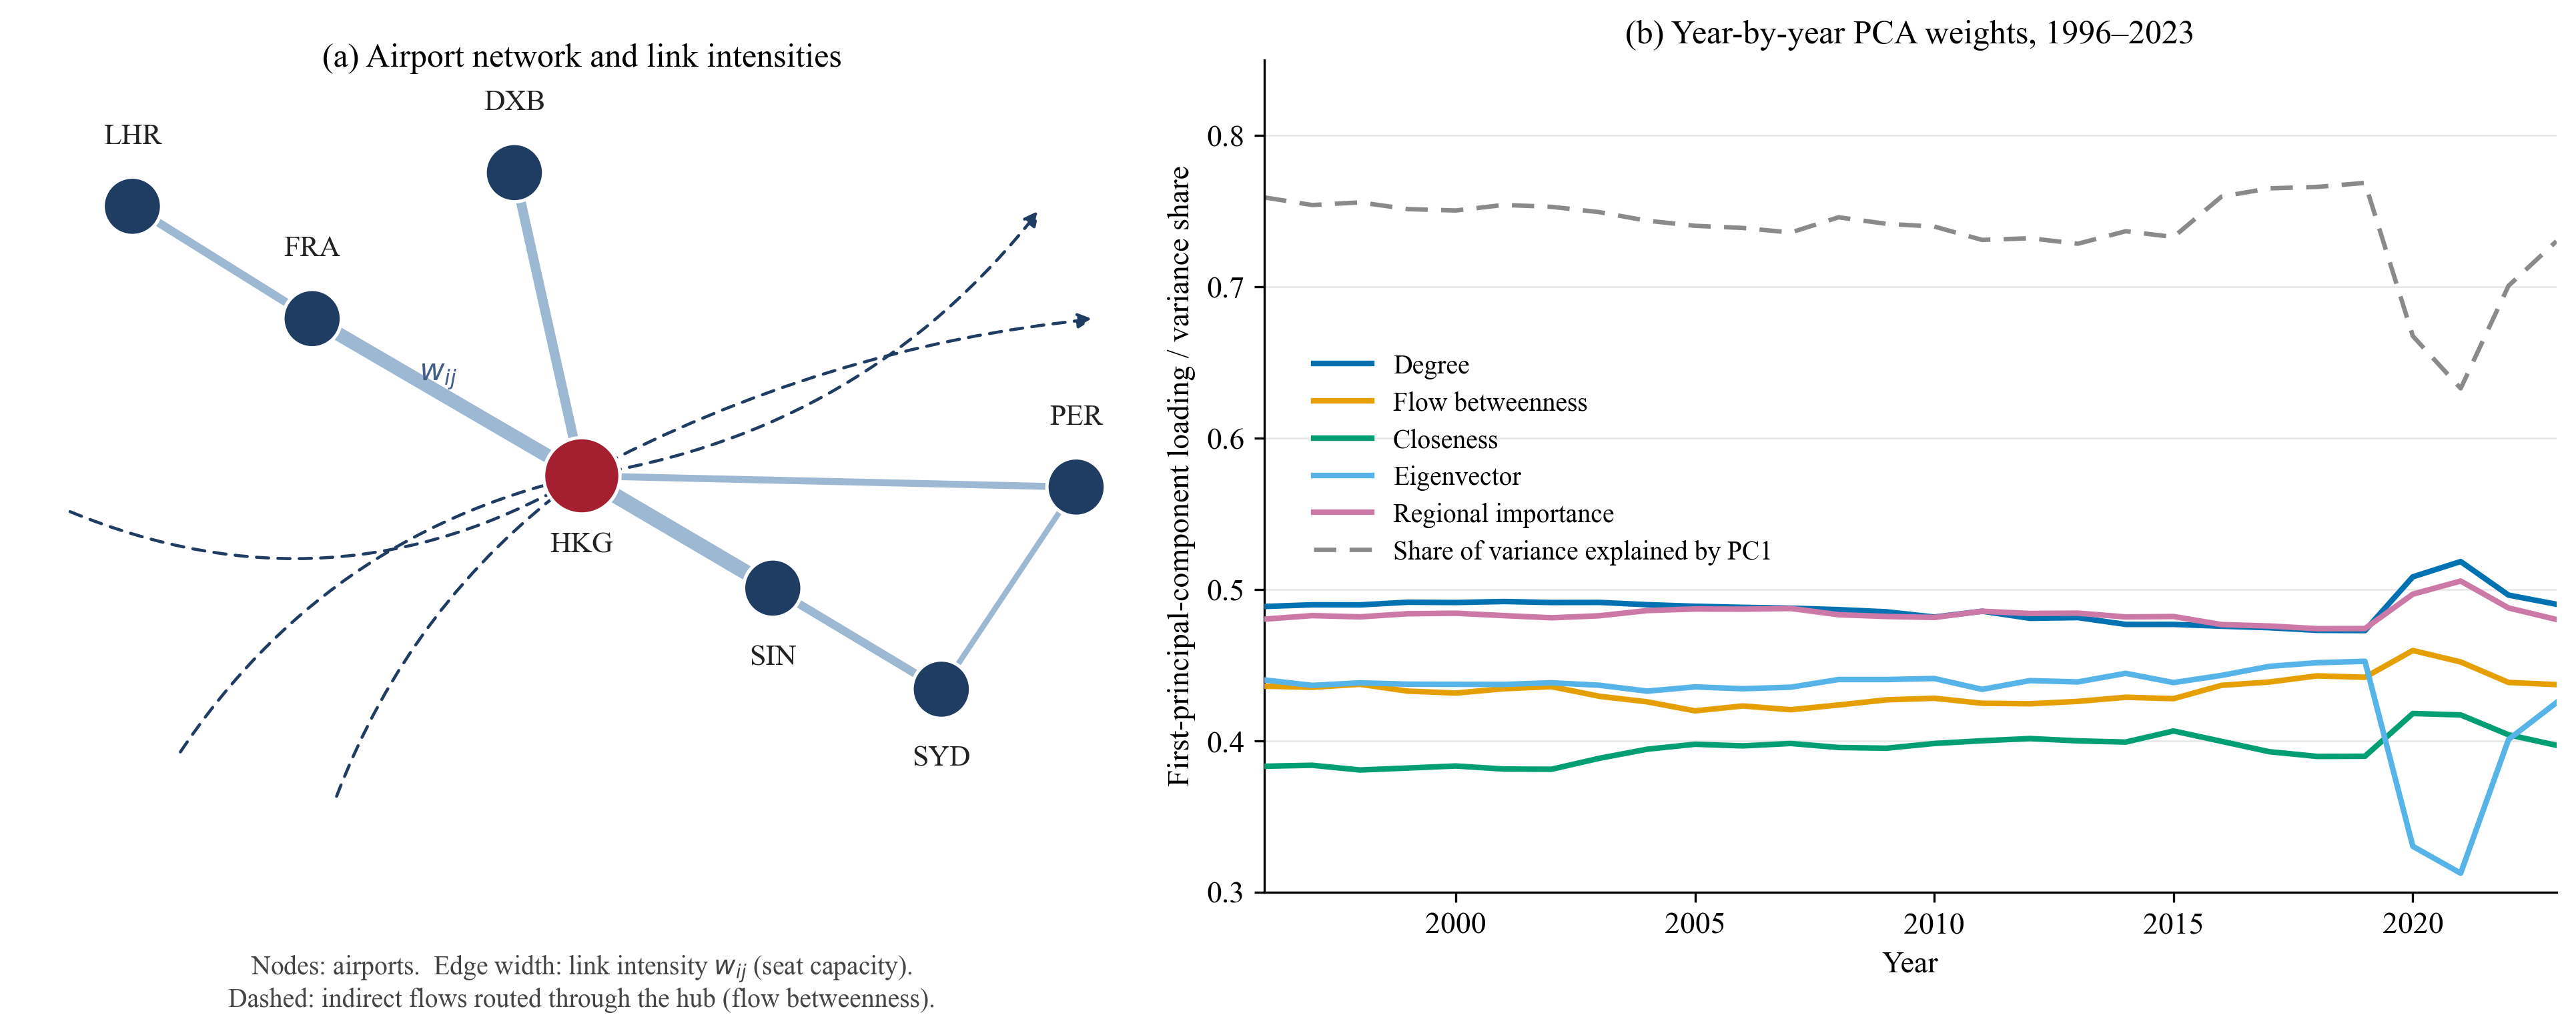
\includegraphics[width=\textwidth]{GACI_method_construction.png}
\caption{Construction of the GACI. Panel (a): schematic airport network,
adapted from \citet{Cheung_2020}. Nodes are airports, edge width is the
link intensity $w_{ij}$ built from scheduled seat capacity
(Eq.~\ref{eq:gaci_link_intensity}), and dashed paths are indirect flows
routed through the hub, which the flow-betweenness indicator captures.
Panel (b): first-principal-component loadings of the five standardised
indicators, re-estimated for each annual network (Eq.~\ref{eq:gaci_pca}),
together with the share of variance explained by the first component.
Loadings are uniformly positive and stable across three decades; the
eigenvector loading dips during the COVID-19 network contraction of
2020--2021 and recovers thereafter.}
\label{fig:gaci_construction}
\end{figure}

For the country-level analysis, airport-level GACI is summarised using three alternative measures. Let $A_{ct}$ denote the set of country $c$'s airports active in year $t$, and let $s_{it}$ denote airport $i$'s total annual scheduled seat capacity, as defined above. The three country-level measures are defined as follows:
\begin{subequations}
\begin{align}
    \mathrm{GACI}_{cwm,ct}
    &=
    \frac{\sum_{i\in A_{ct}} s_{it}\,\mathrm{GACI}_{it}}
         {\sum_{i\in A_{ct}} s_{it}},
    \label{eq:gaci_cwm}\\
    \mathrm{GACI}_{max,ct}
    &=
    \max_{i\in A_{ct}}\mathrm{GACI}_{it},
    \label{eq:gaci_max}\\
    \mathrm{GACI}_{sum,ct}
    &=
    \sum_{i\in A_{ct}}\mathrm{GACI}_{it}.
    \label{eq:gaci_sum}
\end{align}
\end{subequations}
The capacity-weighted mean, $\mathrm{GACI}_{cwm,ct}$, is our headline measure of national ``hub quality'' and uses the entire airport system while placing greater weight on airports carrying more scheduled seat capacity. $\mathrm{GACI}_{max,ct}$ captures the quality of the country's primary gateway, while $\mathrm{GACI}_{sum,ct}$ captures total airport-system connectivity. Figure~\ref{fig:gaci_rankings} reports the rankings the index implies at the airport and the country level, and how they have shifted since 1996.

\begin{figure}[H]
\centering
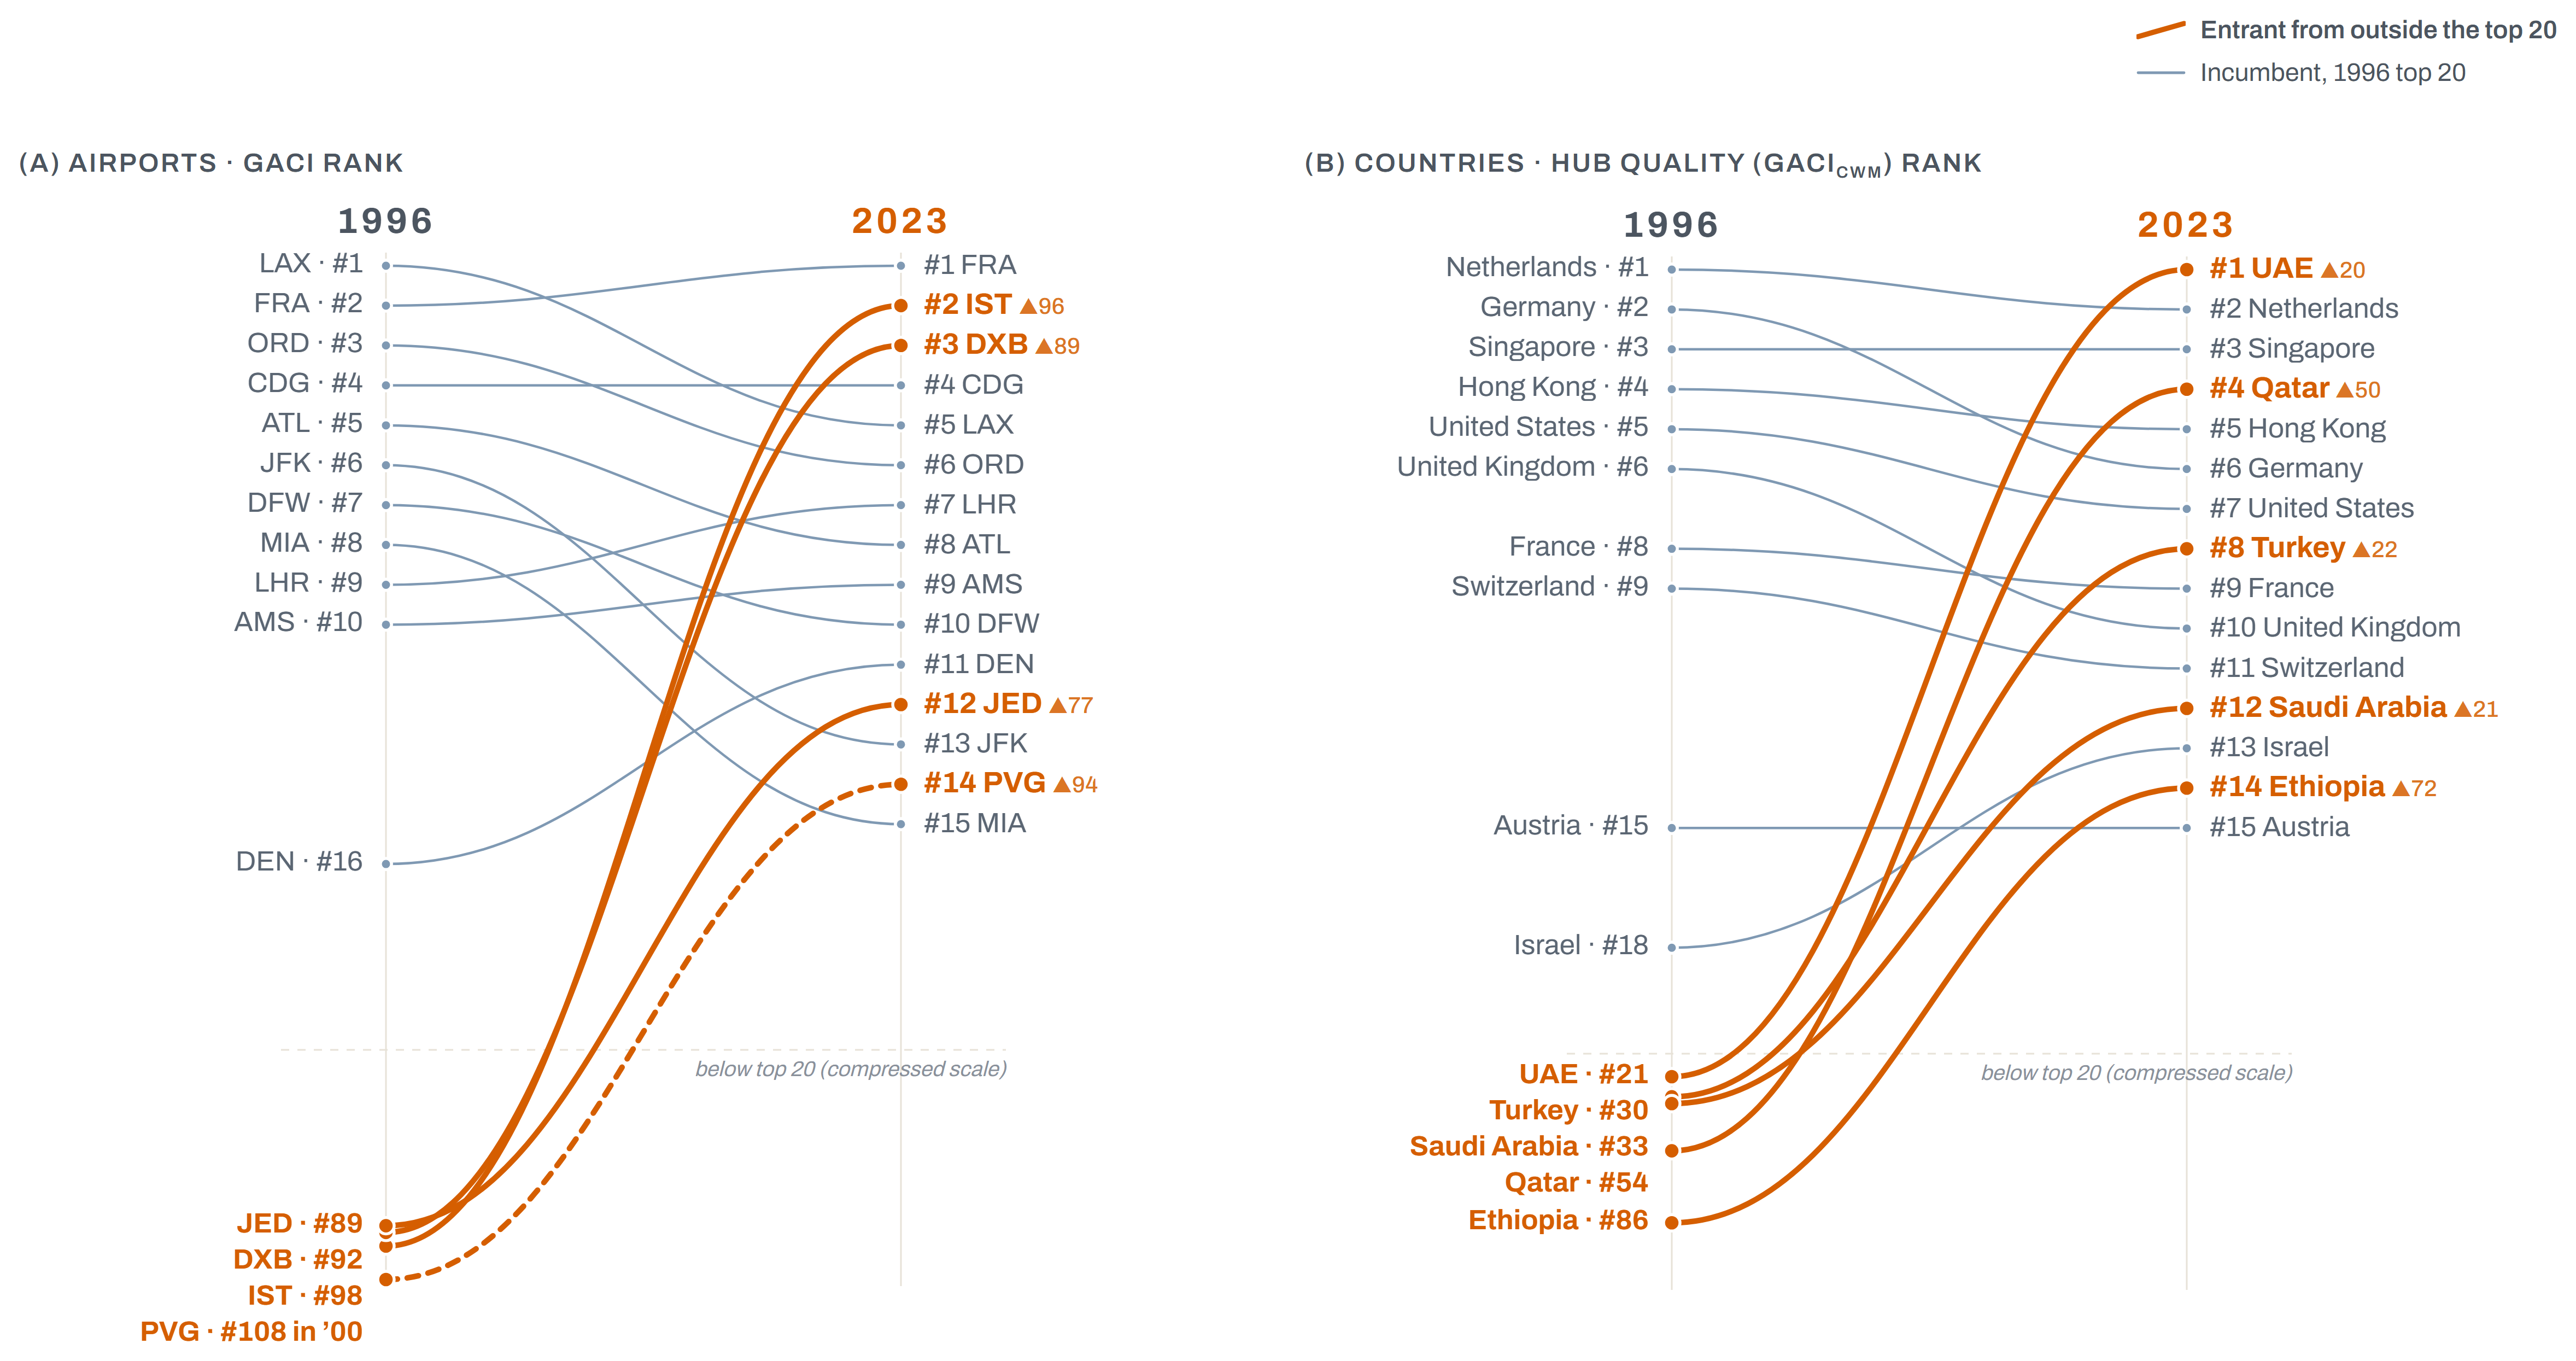
\includegraphics[width=\textwidth]{GACI_rank_bump_rev.png}
\caption{Rank trajectories implied by the index, 1996--2023. Panel (a):
airport-level GACI rank, for the fifteen highest-ranked airports of 2023;
panel (b): country-level hub quality ($\mathrm{GACI}_{cwm}$) rank, for the
fifteen highest-ranked countries of 2023. Country ranks are computed from
the full airport network (all economies with scheduled service), so data
availability in the estimation sample plays no role. Ranks beyond 20 are
drawn on a compressed scale below the dashed divider. Highlighted
trajectories mark entrants from outside the top 20 in 1996, with the number
of places gained shown next to the 2023 label; Shanghai Pudong (PVG,
dashed) enters the network in 2000. The
rise of Gulf and Turkish hubs (Istanbul, Dubai, Jeddah; the United Arab
Emirates, Qatar, Turkey, Saudi Arabia) concentrates after 2010, consistent
with the temporal placement of the identifying variation documented in
Section~\ref{sec:temporal}.}
\label{fig:gaci_rankings}
\end{figure}

As a continuous measure of network connectivity, GACI offers clear advantages over event-based indicators that rely on binary measures of airport or route openings and closures. Binary indicators record only whether a discrete network change occurs and therefore cannot capture adjustments in the intensity of existing services or distinguish changes that differ substantially in scale and network importance. By contrast, GACI jointly reflects the number and strength of connections, the centrality of connected airports, and the indirect accessibility provided by their onward networks. It therefore captures both extensive-margin changes in network coverage and intensive-margin adjustments in flight frequency and seat capacity, providing a more complete measure of the level and evolution of aviation connectivity over time.

\paragraph{\textbf{Outcome}} The outcome is goods (merchandise) trade, measured as
exports plus imports of goods relative to GDP (World Bank WDI,
\texttt{TG.VAL.TOTL.GD.ZS}). The restriction to merchandise is deliberate. The series covers trade in physical goods only, whereas tourist spending is
recorded in the balance of payments as a services export (travel receipts)
and therefore never enters the outcome. In this sense services and tourism
receipts are excluded by construction: any mechanical link from tourist
spending to the outcome is severed at the measurement stage rather than
assumed away (Section~\ref{sec:robust}). From this series we form
three outcomes: log goods volume $\ln g$ (the share multiplied by GDP), log
goods openness $\ln(g/Y)$, and log GDP $\ln Y$. The three are linked by the
identity $\ln g = \ln(g/Y) + \ln Y$, so the volume elasticity decomposes
exactly into an openness component and a scale component. We estimate all
three because each answers a distinct economic question: the volume elasticity measures the total effect of connectivity on trade, the openness elasticity asks whether connectivity makes a country trade more relative to the size of its economy, which is integration proper, and the GDP elasticity asks whether it instead operates by making the economy larger. Reporting all three thus separates two readings of the same headline number, deeper integration versus greater scale.

\paragraph{\textbf{Product-level trade (BACI)}} The WDI outcome is a single
country-year total and cannot reveal which goods respond. For the mechanism
analysis we therefore use BACI (Base pour l'Analyse du Commerce
International), the product-level trade database built by CEPII, the French
research centre for international economics \citep{Gaulier_2010}. Its raw
input is United Nations customs records, in which every trade flow is
reported twice, once by the exporter and once by the importer, with frequent
disagreement between the two; BACI reconciles the mirror reports into a
single value per exporter, importer, product, and year at the six-digit
level of the Harmonized System (HS), the international product nomenclature
of roughly 5{,}000 categories, covering about 200 countries. We aggregate
these bilateral flows to country-year trade values along two product
groupings. The first is unit value: trade value divided by shipped weight
(US dollars per kilogram), with products split at the pooled median: the
median unit value is computed once from all product observations pooled
over the full sample period, rather than year by year, so each product's
classification as high or low unit value is fixed over time. The split is a
standard proxy for whether a good's value-to-weight ratio makes air
shipment economical. The second is end use, using the United Nations Broad
Economic Categories (BEC) correspondence to separate intermediate inputs
from final consumption goods; capital goods, which the BEC assigns to an
end-use class of their own, are grouped separately and do not enter the
intermediate-to-consumption ratio. Summed over all products, BACI trade closely
tracks the WDI outcome (within-country correlation $0.80$); the correlation
falls short of unity because the two sources differ in reporting basis and
coverage, with BACI reconciling customs records while the WDI merchandise
series follows balance-of-payments conventions, so the disaggregation
refines rather than replaces the headline measure.

\paragraph{\textbf{Instrument variable}} We instrument connectivity with a shift-share
interaction of a predetermined national exposure and a global demand shock.
The design has a lineage: UNESCO World Heritage listings have been used to
instrument tourism specialisation in cross-country growth regressions
\citep{Arezki_2009}, and coastal geography has served as exogenous tourism
attractiveness in within-country designs \citep{Faber_2019}. The fixed
``share'' is each country's cumulative count of natural and mixed
UNESCO World Heritage sites, endowments rooted in geography rather than in
economic activity. The global ``shift'' is world international tourist
arrivals (WDI \texttt{ST.INT.ARVL}, 1996--2019; extended to 2020--2023 with
UNWTO figures), min--max scaled to $[0,1]$. The baseline instrument is
\begin{equation}
\text{tourism\_int}_{ct}
= \underbrace{\widetilde{D}_t}_{\text{global tourism shift}}
\times \underbrace{\ln\!\bigl(1+H_c^{\text{nat+mix}}\bigr)}_{\text{fixed heritage share}}.
\label{eq:instr}
\end{equation}
The identifying variation is differential, and the economic mechanism behind it is the route-allocation calculus of airlines. Carriers deploy marginal aircraft and frequencies where expected passenger demand is
highest, and when the global tourism cycle rises, expected leisure demand rises most in destinations with strong natural attractions. Natural and mixed World Heritage sites provide a predetermined, internationally
certified marker of that leisure attractiveness, so heritage-rich countries receive a disproportionate share of tourism-driven route and capacity growth, shifting their network position for reasons unrelated to their
contemporaneous goods-trade shocks. Natural heritage serves as the exposure measure precisely because it is rooted in physical geography (reefs, mountain ranges, national parks) rather than in economic activity. Unlike
cultural sites, whose listing tracks historical development and urbanisation, a country's endowment of natural sites is not itself a product of its trading economy. Country fixed effects absorb the level of the heritage endowment and year fixed effects absorb the global shift itself, so only the interaction identifies. In the language of the shift-share literature, the identifying assumption is exogeneity of the predetermined shares \citep{GoldsmithPinkham_2020}, while the common shift requires no exogeneity of its own because year fixed effects absorb it \citep{Borusyak_2022}. The exclusion restriction is that heritage-driven tourism demand affects goods trade only through air connectivity. The maintained channel, that air links build trade through business travel, face-to-face contact, and access to distant inputs, is itself well documented \citep{Campante_2017,Feyrer_2019}. Two design choices narrow the space of violations from the outset. First, the outcome excludes services and tourism receipts, cutting the most direct alternative channel. The prominent remaining path, tourism-driven real-exchange-rate appreciation that crowds out tradable production \citep{Copeland_1991,Holzner_2011}, works against the positive elasticities we estimate, and any income-mediated import demand is bounded by conditioning on GDP (Table~\ref{tab:controls}). Second, cultural sites, which co-move with historical development and whose listing is most exposed to political influence \citep{Bertacchini_2016}, are deliberately left out of the share.
\ref{sec:robust} presents the full validity battery, including a falsification test that lets the data reject cultural heritage as an instrument, and an independent air/sea-distance instrument built from geography and the CERDI sea-distance database \citep{Bertoli_2016}.

\paragraph{\textbf{Sample}} An unbalanced panel of 184 countries observed annually from 1996 to 2023, with 4{,}643 of the $184\times28=5{,}152$ possible country-year observations. 136 of the 184 countries are observed in all 28
years. The gaps arise almost entirely from missing WDI merchandise-trade or
GDP entries, concentrated in small island economies and conflict-affected
states, with a residual handful of country-years in which no scheduled air
service operated (for example, Iraq in 1996--2004). One country (New
Caledonia) enters with a single observation, which the country fixed effect
absorbs, so the regressions use 4{,}642 observations. Table~\ref{tab:sumstat}
reports summary statistics. Goods trade averages 66\% of GDP (median 56\%). Air-network
position is highly skewed: the median country operates 5 airports with active
scheduled service while the largest reaches 614, and the median country holds a
single natural or mixed UNESCO site while the most heritage-rich holds eighteen.
Summary statistics are reported in natural units; monetary and scale variables
enter the regressions in logs, and population is a control.
Figure~\ref{fig:basemap} maps the 2023 cross-section of the index and shows
where this skewness sits geographically: connectivity is concentrated in the
United States and China, followed by the large continental economies (Canada,
Russia, Brazil, India, Indonesia) and the established hub countries of Europe
and East Asia, while the least connected countries are small island states and
parts of sub-Saharan Africa. Because levels differ this widely across
countries, the fixed-effects design draws identification from within-country
changes in connectivity over time rather than from the cross-sectional ranking
the map displays.

\begin{table}[H]
\centering
\caption{Summary statistics, estimation sample (184 countries, 1996--2023).}
\label{tab:sumstat}
\begin{threeparttable}
\small
\begin{tabular}{lrrrrrr}
\toprule
Variable & $N$ & Mean & SD & Min & Median & Max \\
\midrule
\multicolumn{7}{l}{\emph{Connectivity}}\\
Hub quality, $\mathrm{GACI}_{cwm}$ (cap.-wtd.\ mean index) & 4643 & 1.09 & 0.40 & 0.53 & 0.99 & 3.01 \\
Total connectivity, $\mathrm{GACI}_{sum}$ (index) & 4643 & 14.29 & 41.91 & 0.55 & 4.00 & 510.04 \\
Number of airports & 4643 & 19.32 & 52.65 & 1.00 & 5.00 & 614.00 \\
\addlinespace
\multicolumn{7}{l}{\emph{Trade outcomes}}\\
Goods-trade volume (billion USD) & 4643 & 203.5 & 560.1 & 0.06 & 20.9 & 6{,}993.7 \\
Goods trade (\% of GDP) & 4643 & 65.99 & 43.90 & 7.81 & 55.68 & 420.68 \\
\addlinespace
\multicolumn{7}{l}{\emph{Income}}\\
GDP per capita (USD) & 4643 & 14{,}019 & 19{,}173 & 227 & 5{,}059 & 118{,}383 \\
GDP (billion USD) & 4643 & 374.9 & 1{,}573.7 & 0.06 & 27.8 & 27{,}292.2 \\
\addlinespace
\multicolumn{7}{l}{\emph{Instrument and heritage}}\\
Tourism-heritage instrument & 4643 & 0.42 & 0.47 & 0.00 & 0.34 & 2.94 \\
Natural + mixed UNESCO sites (cum.) & 4643 & 1.82 & 2.77 & 0.00 & 1.00 & 18.00 \\
\addlinespace
\multicolumn{7}{l}{\emph{Controls}}\\
Population (million) & 4643 & 39.31 & 144.52 & 0.01 & 8.32 & 1{,}438.07 \\
Land area (thousand km$^2$) & 4643 & 742.8 & 1{,}964.3 & 0.02 & 155.4 & 16{,}388.5 \\
Remoteness, mean sea distance (km) & 4635 & 10{,}800 & 1{,}815 & 7{,}811 & 10{,}592 & 15{,}297 \\
\bottomrule
\end{tabular}
\begin{tablenotes}\small
\item All variables are reported in natural units; monetary values are in
current US dollars. Goods trade is merchandise trade (WDI); services and
tourism are excluded by construction. The regressions use logs of the
monetary and scale variables; the outcome goods openness is constructed from
the Goods trade (\% of GDP) series as
$\ln(\text{goods}/\text{GDP})=\ln(\text{share}/100)$. Hub quality is the
capacity-weighted mean of airport-level
GACI; total connectivity is the country sum. The tourism-heritage instrument is
global tourism demand (min--max scaled) interacted with the fixed
natural-plus-mixed heritage endowment.
\end{tablenotes}
\end{threeparttable}
\end{table}


\begin{figure}[H]
\centering
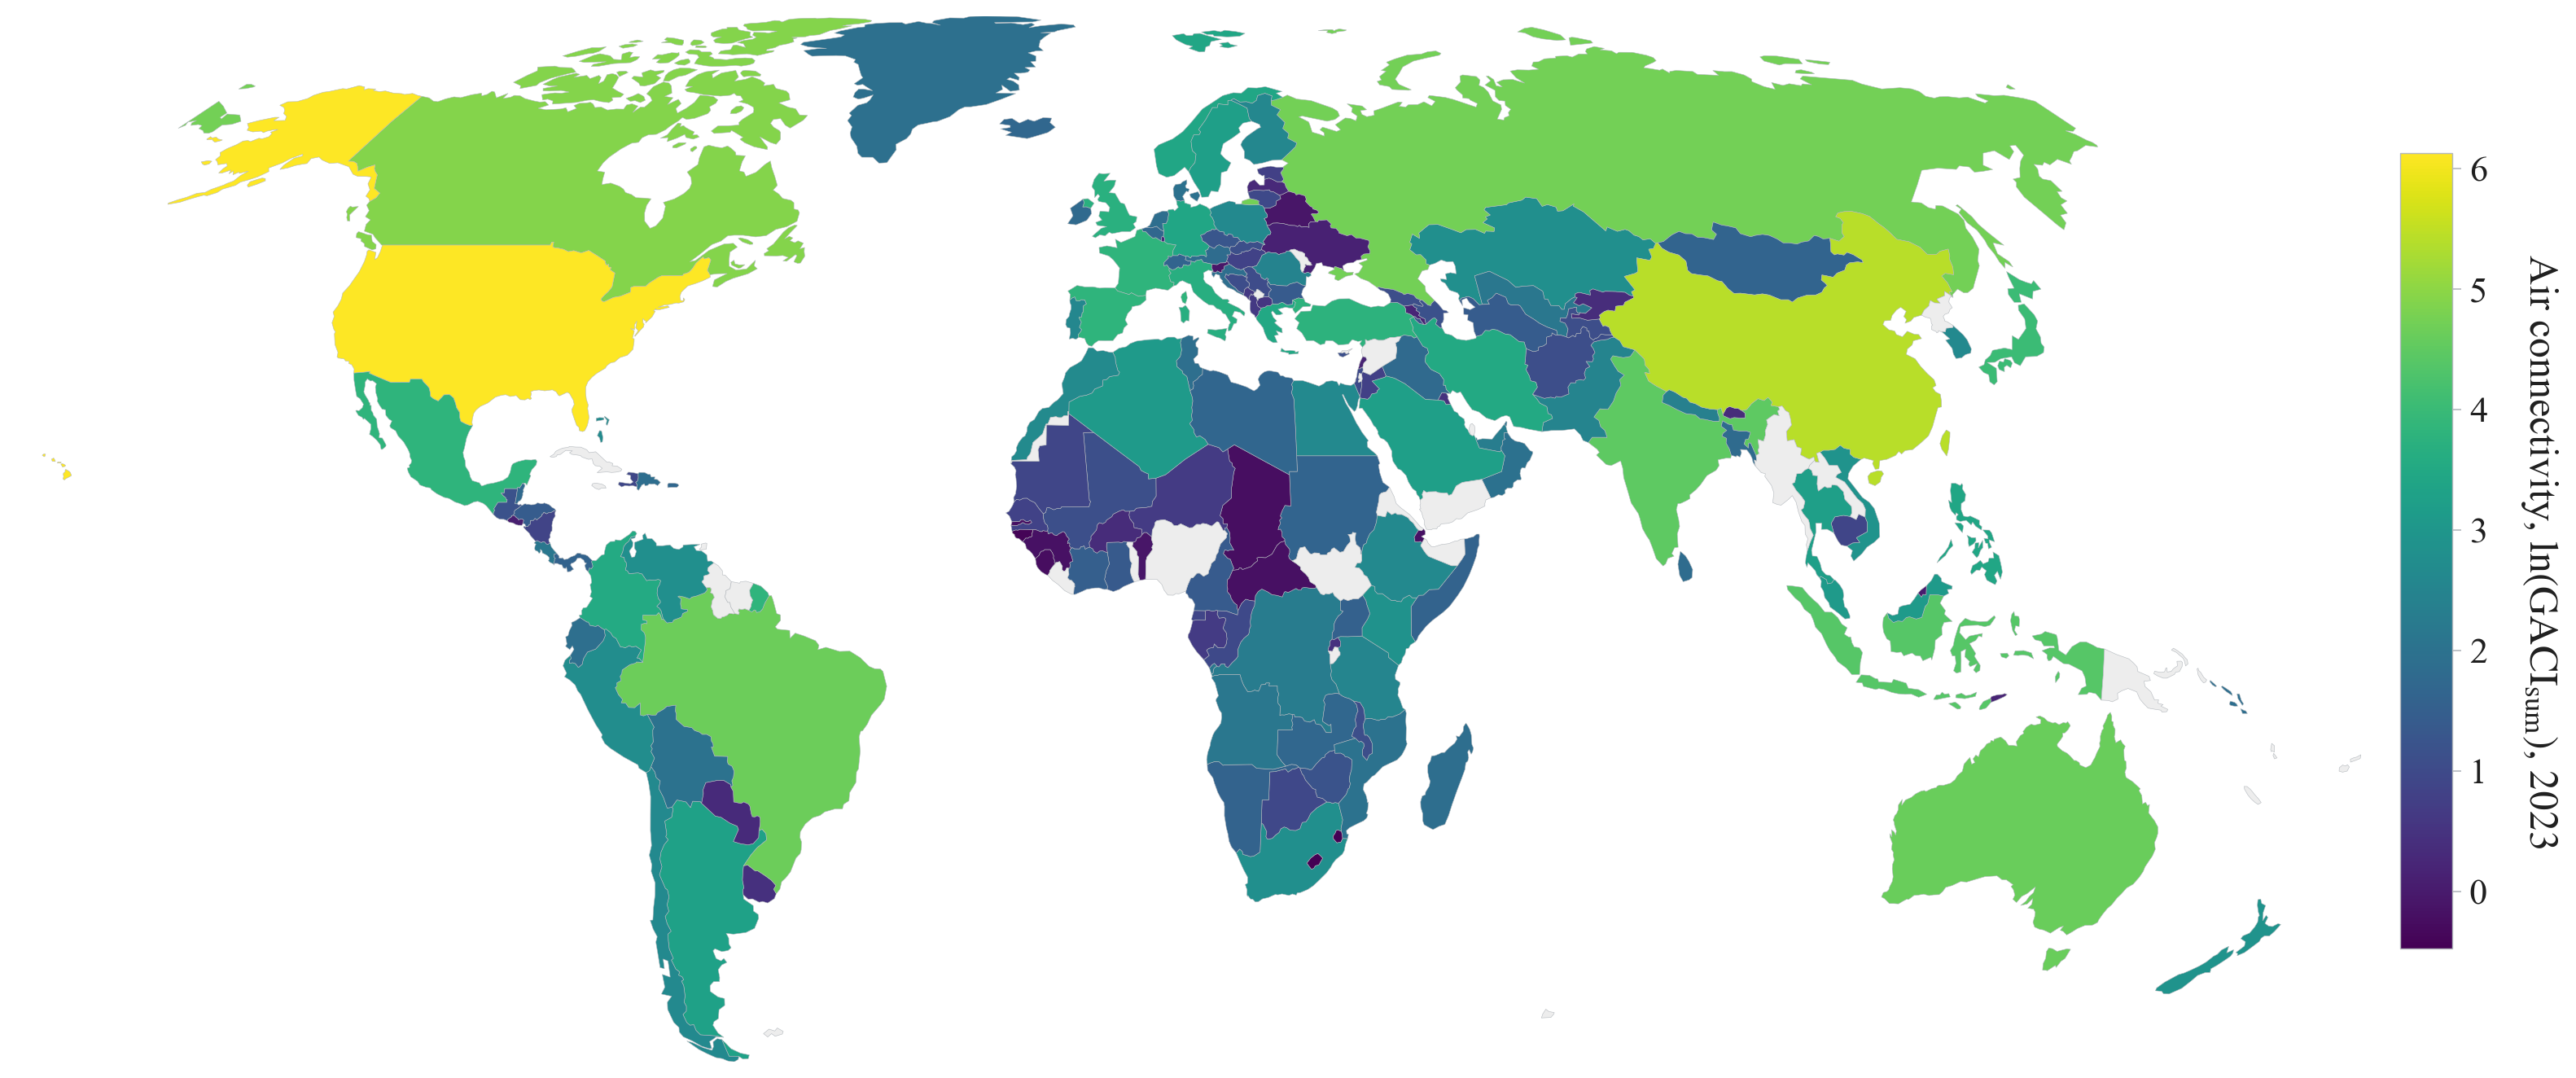
\includegraphics[width=0.9\linewidth]{GACI_base_map.png}
\caption{Air connectivity (GACI) levels, 2023. Yellow = highly connected
(United States, China, large European hubs).}
\label{fig:basemap}
\end{figure}
%=======================================================================
\section{Empirical strategy}
\label{sec:strategy}
%=======================================================================
To estimate the impact of GACI on trade openness, we estimate the following model:

\begin{equation}
y_{ct} = \beta\,\ln\mathrm{GACI}_{ct} + \gamma\,\ln\text{pop}_{ct}
+ \alpha_c + \delta_t + \varepsilon_{ct},
\label{eq:main}
\end{equation}

where $y_{ct}$ denotes trade and economic outcomes, including the natural logarithm of trade volume ($\ln g$), GDP ($\ln y$), and trade openness ($\ln (g/y)$) for country $c$ in year $t$. $\ln \mathrm{GACI}_{ct}$ represents the natural logarithm of GACI for country $c$ in year $t$. We consider three alternative measures of GACI: (i) \textit{hub quality} ($GACI_{cwm, ct}$), defined as the capacity-weighted mean of airport-level GACI within country $c$; (ii) the maximum airport-level GACI in country $c$  ($GACI_{max, ct}$); and (iii) the total GACI, calculated as the sum of airport-level GACI values within country $c$  ($GACI_{sum, ct}$). We also control for the natural logarithm of population. The model includes country fixed effects ($\alpha_c$) and year fixed effects ($\delta_t$). Population is the only time-varying control in the baseline for a deliberate reason: the country fixed effects absorb all time-invariant determinants of trade, and the natural time-varying candidates, GDP and income, are themselves outcomes of connectivity (Table~\ref{tab:main}), so conditioning on them would control away part of the effect of interest. Population, by contrast, is a standard scale control for trade openness that is plausibly unaffected by connectivity at annual frequency. Table~\ref{tab:controls} shows that the headline estimate is insensitive to adding these richer control sets.

Identifying the causal effect of connectivity on trade is difficult for two
reasons. First, connectivity is poorly represented by a binary treatment. New
airports and major international routes open only rarely and lumpily, and a
country's effective network position evolves continuously, through
frequencies, partner growth, and re-routing, rather than through discrete,
datable openings; the discrete events that could anchor a staggered
difference-in-differences design are both scarce and a coarse proxy for the
connectivity that actually changes. Second, the variation that does exist is
endogenous: airlines add capacity where trade and income are already growing.
The first consideration motivates the measurement choice, and we address it
with a continuous, network-based index that embeds second-order
(partner-of-partner) spillovers. The second consideration, endogeneity, is
what necessitates instrumental variables, and we instrument connectivity with
a shift-share interaction
\citep{GoldsmithPinkham_2020,Borusyak_2022} of a fixed heritage endowment with
the global tourism cycle. Heritage-driven leisure demand shifts an airport's
network position for reasons unrelated to goods-trade fundamentals, while the
outcome excludes services and tourism by construction; this removes the
mechanical channel from tourist spending to the outcome, though indirect
channels from tourism demand to merchandise trade remain possible and are
examined in \ref{sec:robust}. We report
heteroskedasticity-robust standard errors and probe the exclusion restriction
through over-identification and falsification tests (\ref{sec:robust}); such
tests can detect violations but cannot establish the restriction, which
remains an identifying assumption.

Using the instrumental variable, $\text{tourism\_int}_{ct}$, we estimate the model using two-stage least squares (2SLS). The first-stage regression is specified as follows:

\begin{equation}
\ln\mathrm{GACI}_{ct} = \pi_1\text{tourism\_int}_{ct} + \pi_2\ln\text{pop}_{ct} +  \mu_c + \lambda_t + \nu_{ct}.
  \label{eq:first}
  \end{equation}

Using the predicted values, $\widehat{\ln\mathrm{GACI}}_{ct}$, obtained from Equation \eqref{eq:first}, we then estimate the second-stage regression given by Equation \eqref{eq:main}.

For additional analyses, we examine (1) heterogeneity in the effects of GACI, (2) the mechanisms through which GACI affects trade openness, and (3) the aggregate contribution of GACI to trade over the period 1996--2023.

For (1), we investigate heterogeneous effects of GACI using the following interaction model:

\begin{equation}
y_{ct} = \beta_1\,\ln\mathrm{GACI}_{ct}
+\beta_3\,\bigl(\ln\mathrm{GACI}_{ct} \times \mathrm{Moderator}_{c}\bigr)
+ \gamma\,\ln\mathrm{pop}_{ct}
+ \alpha_c + \delta_t + \varepsilon_{ct},
\label{eq:mod}
\end{equation}

where $\mathrm{Moderator}_{c}$ denotes the moderator variable. We consider three moderators, all country-specific and time-invariant: the mean-centred baseline value of the natural logarithm of GDP per capita, baseline global connectivity ($\ln\mathrm{GACI}_{\mathrm{cwm},c,1996}$), and remoteness, defined as each country's unweighted mean sea distance to all other sample countries, from the CERDI sea-distance database \citep{Bertoli_2016}, in logs. Because the moderators do not vary over time, their main effects are absorbed by the country fixed effects $\alpha_c$ and cannot be separately identified, so Equation~\eqref{eq:mod} contains only the connectivity term and its interaction. Both $\ln\mathrm{GACI}_{ct}$ and the interaction term are treated as endogenous and instrumented with the corresponding pair of instruments, $\text{tourism\_int}_{ct}$ and $\text{tourism\_int}_{ct}\times\mathrm{Moderator}_{c}$. The interaction terms allow us to estimate how the effect of $\ln\mathrm{GACI}_{\mathrm{cwm},ct}$ varies across these dimensions. In addition, we examine temporal heterogeneity by estimating the model separately for the pre-2010 and post-2010 periods.

For (2), we investigate the mechanisms underlying the effect of GACI on trade openness. We consider two potential mechanism variables, each capturing a compositional margin of trade. The first is the log ratio of intermediate-goods trade volume to consumption-goods trade volume,
$\mathrm{M}_{ct} = \ln \left( \frac{\mathrm{Interm.}_{ct}}{\mathrm{Consum.}_{ct}} \right)$,
which captures the value-chain margin. The second is the log ratio of high- to low-unit-value trade,
$\mathrm{M}_{ct} = \ln \left( \frac{\mathrm{High\ UV}_{ct}}{\mathrm{Low\ UV}_{ct}} \right)$,
which captures the air-freight margin. For each mechanism variable $\mathrm{M}_{ct}$ so defined, we estimate the following equations:

\begin{equation}
\mathrm{M}_{ct}
= \kappa_1\,\ln\mathrm{GACI}_{ct}
+ \kappa_2\,\ln\mathrm{pop}_{ct}
+ \xi_c + \zeta_t + \phi_{ct},
\label{eq:mec1}
\end{equation}

\begin{equation}
y_{ct}
= \beta_1\,\ln\mathrm{GACI}_{ct}
+ \beta_2\,\mathrm{M}_{ct}
+ \gamma\,\ln\mathrm{pop}_{ct}
+ \alpha_c + \delta_t + \varepsilon_{ct}.
\label{eq:mec2}
\end{equation}

In Equations~\eqref{eq:mec1} and \eqref{eq:mec2}, statistically significant estimates of both $\kappa_1$ and $\beta_2$ constitute evidence consistent with GACI operating on trade openness through the corresponding compositional margin. We emphasise that this is a descriptive decomposition rather than a formal causal mediation analysis. The mechanism variable $\mathrm{M}_{ct}$ is itself an outcome of connectivity and is then included as a regressor in Equation~\eqref{eq:mec2}, so without additional identifying assumptions for the mediator, $\beta_1$ should be read as the connectivity coefficient conditional on the composition margin, not as a structural ``direct effect.'' Similarly, because unobserved factors may move both the composition ratio and openness, a statistically significant $\beta_2$ establishes an association between composition and openness rather than a causal effect of the composition margin itself. We therefore interpret the results of this exercise as suggestive evidence on the compositional channel, consistent with the limitation acknowledged in Section~\ref{sec:discussion}.

For (3), we quantify the aggregate contribution of GACI by converting the estimated elasticity of trade openness with respect to GACI into implied dollar changes in trade for each country (Section~\ref{sec:aggregate}).

%=======================================================================
\section{Main results}
\label{sec:results}
%=======================================================================

We first ask whether global aviation connectivity raised trade openness, trade
volume, and GDP. Table~\ref{tab:main} reports, for each of our three measures of
global aviation connectivity, three lines side by side: the OLS association, the
first-stage relevance of the instrument, and the instrumented (2SLS) estimate.
Reading down each panel shows how isolating exogenous variation changes the
picture. The three measures agree closely in sign and significance, so we adopt
hub quality ($\ln\mathrm{GACI}_{cwm}$) as our main explanatory variable: unlike
the maximum, which discards every airport but the primary gateway, and the simple
sum, which weights a minor regional field the same as a major hub, the
capacity-weighted mean uses the entire airport system while still placing most
weight on the dominant hubs. We therefore report hub quality in Panel~A and treat
the maximum and the sum as robustness measures.

Panel A uses hub quality ($\ln\mathrm{GACI}_{cwm}$), our headline measure, as the independent variable. The
instrument is a strong predictor of connectivity: it enters the first stage with
the expected positive sign ($0.032$, $p<0.01$), and the Kleibergen--Paap
statistic ($F=18.0$) sits comfortably above conventional weak-instrument
thresholds. In the second stage, a one-percent increase in hub quality raises
trade volume by about $2.3\%$ ($p<0.01$). This volume response decomposes into two
parts. Trade openness, the ratio of trade to GDP, rises by about $1.3\%$
($p<0.05$), and GDP rises by about $1.0\%$, although the GDP estimate is not
statistically significant. We treat trade openness as the headline result because
it isolates the pure trade effect net of economic scale. It measures whether
connectivity makes a country trade more relative to the size of its economy,
rather than simply enlarging the economy as a whole. These estimates bear
directly on \textbf{Hypothesis~1}, which predicts that higher aviation connectivity
increases merchandise trade. The \textbf{Hypothesis 1} is supported on the volume margin
and, more stringently, on the openness margin net of economic scale.

Panel B introduces the maximum hub measure ($\ln\mathrm{GACI}_{max}$), which keeps
only each country's single best-connected gateway. This is the strongest of the
three instruments: the tourism-heritage instrument enters the first stage at
$0.044$ ($p<0.01$) with a Kleibergen--Paap statistic of $27.4$, the highest in the
table. The second-stage estimates track Panel A in sign and significance, trade
volume rising by about $1.7\%$ ($p<0.01$) and openness by about $1.0\%$
($p<0.05$), while the GDP effect is again positive but not significant. That the
hub-only measure delivers the tightest first stage is consistent with the
hub-and-spoke logic that a country's primary gateway carries most of its
exogenous, tourism-driven connectivity.

Panel C repeats the exercise with total connectivity ($\ln\mathrm{GACI}_{sum}$),
which sums connectivity across all airports and so blends hub quality with sheer
airport count. The qualitative picture is unchanged: volume and openness are
positive and significant, while the GDP effect is positive but imprecise. Its
first stage is the weakest of the three ($F=9.7$), as expected once hub
concentration is diluted by peripheral airports. The three measures are on
different scales and cannot be compared coefficient for coefficient. What carries
over is the common pattern of signs and significance, together with the exact
decomposition that holds in every panel. The support for \textbf{Hypothesis~1} is
therefore not an artefact of any one aggregation of connectivity.

\begin{table}[H]
\centering
\caption{Main results: OLS, first stage, and 2SLS, by connectivity measure (robust SE).}
\label{tab:main}
\begin{threeparttable}
\small
\begin{tabular}{lccc}
\toprule
 & Trade openness & Trade volume & GDP \\
 & $\ln(g/Y)$ & $\ln g$ & $\ln Y$ \\
\midrule
\multicolumn{4}{l}{\emph{Panel A. Hub quality, $\ln\mathrm{GACI}_{cwm}$ (headline)}}\\
First stage: instrument coef. & \multicolumn{3}{l}{0.032\sym{***}\ \ (0.007),\ \ KP $F=18.0$} \\
OLS & 0.157\sym{***} & 1.144\sym{***} & 0.987\sym{***} \\
2SLS & 1.302\sym{**} & 2.303\sym{***} & 1.001 \\
 & (0.662) & (0.776) & (0.680) \\
\addlinespace
\multicolumn{4}{l}{\emph{Panel B. Maximum hub, $\ln\mathrm{GACI}_{max}$}}\\
First stage: instrument coef. & \multicolumn{3}{l}{0.044\sym{***}\ \ (0.008),\ \ KP $F=27.4$} \\
OLS & 0.103\sym{**} & 1.083\sym{***} & 0.980\sym{***} \\
2SLS & 0.966\sym{**} & 1.709\sym{***} & 0.743 \\
 & (0.469) & (0.548) & (0.507) \\
\addlinespace
\multicolumn{4}{l}{\emph{Panel C. Total connectivity, $\ln\mathrm{GACI}_{sum}$}}\\
First stage: instrument coef. & \multicolumn{3}{l}{0.064\sym{***}\ \ (0.020),\ \ KP $F=9.7$} \\
OLS & -0.027 & 0.237\sym{***} & 0.264\sym{***} \\
2SLS & 0.659\sym{*} & 1.166\sym{***} & 0.507 \\
 & (0.365) & (0.432) & (0.341) \\
\midrule
Country, Year FE & Yes & Yes & Yes \\
Observations & 4{,}642 & 4{,}642 & 4{,}642 \\
\bottomrule
\end{tabular}
\begin{tablenotes}\small
\item Robust (heteroskedasticity-consistent) SE in parentheses. Each panel
instruments its connectivity measure with the tourism-heritage instrument. The
first-stage row regresses the connectivity measure on the instrument (with
population and two-way FE); KP $F$ is the Kleibergen--Paap first-stage statistic.
Trade volume $=$ openness $+$ GDP by the identity $\ln g=\ln(g/Y)+\ln Y$.
\sym{*}~$p<0.10$, \sym{**}~$p<0.05$, \sym{***}~$p<0.01$.
\end{tablenotes}
\end{threeparttable}
\end{table}
%=======================================================================
\subsection{Heterogeneity: who gains most?}
%=======================================================================

We next ask whether the average effect masks variation in who benefits, letting
the connectivity elasticity vary with three mean-centred baseline moderators:
income (log GDP per capita), global aviation connectivity ($\ln\mathrm{GACI}_{cwm}$),
and remoteness. Remoteness is each country's unweighted mean sea distance to all
other sample countries, from the CERDI sea-distance database, in logs. It is a
time-invariant, purely geographic measure (we use the unweighted mean because
GDP-weighting collapses to market proximity and inverts the ranking).
Table~\ref{tab:het} reports interaction-IV estimates: for each moderator,
``$\ln\mathrm{GACI}_{cwm}$ (at mean)'' is the effect for the average country and
``$\times$ moderator'' is how that effect shifts as the moderator rises, with both
the connectivity term and its interaction instrumented.

The interactions with baseline income and baseline connectivity are negative and
significant across all three outcomes: the payoff to connectivity is larger in
poorer and less-connected economies. The remoteness interaction is also negative
for openness, but because remoteness is measured as mean sea distance, the sign
here has the opposite substantive reading: the openness payoff is, if anything,
larger for less remote economies, and the interaction is imprecise for volume
and GDP. Evaluated at the mean the effect remains positive and sizeable. The
interacted first stages are weaker (KP $F\approx5$--$9$), so we read the gradient
as a qualitative pattern and report every cell.\footnote{Three considerations
discipline this reading. First, the conventional rule of thumb of ten is
calibrated to a single endogenous regressor, whereas
Equation~\eqref{eq:mod} instruments two terms; because both instruments are
built from a single underlying shifter, the two instrumented terms are highly
correlated, which mechanically depresses the joint Kleibergen--Paap statistic
even when each instrument is individually relevant. Second, the level of the
gradient is anchored by the uninteracted specification, whose first stage is
strong (KP $F=18.0$, Table~\ref{tab:main}); what the weaker interacted stage
puts at risk is the precision of the slope, and the sign pattern is consistent
across all three moderators and all three outcomes. Third, the interacted
instruments inherit the exogeneity of the baseline instrument, since they
multiply it by predetermined, time-invariant country characteristics: the
modest $F$ is a question of statistical power, not of identification, and its
cost, wide confidence intervals, is visible in the table.}

\begin{table}[H]
\centering
\caption{Heterogeneity: interaction IV (robust SE).}
\label{tab:het}
\begin{threeparttable}
\small
\begin{tabular}{lccc}
\toprule
Moderator (mean-centred): & Baseline income & Baseline conn. & Remoteness \\
\midrule
\multicolumn{4}{l}{\emph{Panel A. Trade openness $\ln(g/Y)$}}\\
$\ln\mathrm{GACI}_{cwm}$ (at mean)   & 1.254\sym{*}  & 2.260\sym{*}  & 1.391\sym{**} \\
                         & (0.717)       & (1.161)       & (0.693) \\
$\times$ moderator       & $-0.243$\sym{**} & $-1.482$\sym{**} & $-1.241$\sym{*} \\
                         & (0.122)       & (0.622)       & (0.673) \\
\addlinespace
\multicolumn{4}{l}{\emph{Panel B. Trade volume $\ln g$}}\\
$\ln\mathrm{GACI}_{cwm}$ (at mean)   & 1.959\sym{***} & 6.093\sym{***} & 2.394\sym{***} \\
                         & (0.732)       & (1.742)       & (0.825) \\
$\times$ moderator       & $-1.108$\sym{***} & $-6.060$\sym{***} & $-1.234$ \\
                         & (0.131)       & (1.046)       & (0.815) \\
\addlinespace
\multicolumn{4}{l}{\emph{Panel C. GDP $\ln Y$}}\\
$\ln\mathrm{GACI}_{cwm}$ (at mean)   & 0.705         & 3.834\sym{***} & 1.003 \\
                         & (0.759)       & (1.133)       & (0.708) \\
$\times$ moderator       & $-0.865$\sym{***} & $-4.579$\sym{***} & 0.007 \\
                         & (0.119)       & (0.677)       & (0.755) \\
\midrule
First-stage KP $F$       & 8.07          & 4.96          & 9.21 \\
Country, Year FE         & Yes           & Yes           & Yes \\
Observations             & 4{,}121       & 4{,}121       & 4{,}635 \\
\bottomrule
\end{tabular}
\begin{tablenotes}\small
\item Each column is one moderator. Both $\ln\mathrm{GACI}_{cwm}$ and its
interaction with the (mean-centred) moderator are instrumented; country and year
FE; robust SE. Negative interactions mean the payoff is larger for poorer and
less-connected economies; KP $F$ is modest ($\approx5$--$9$), so the gradient is
qualitative. Samples are smaller than in Table~\ref{tab:main}: the baseline
income and connectivity moderators require observation in 1996 (4{,}121), and
sea distance is unavailable for a handful of economies (4{,}635).
\sym{*}~$p<0.10$, \sym{**}~$p<0.05$, \sym{***}~$p<0.01$.
\end{tablenotes}
\end{threeparttable}
\end{table}

Figure~\ref{fig:hetquartile} makes this gradient concrete by plotting the implied
openness elasticity for each quartile of baseline income and baseline
connectivity. In both dimensions the elasticity falls monotonically from the
lowest to the highest quartile, from about $1.7$ to $0.8$ across income quartiles
and from about $2.7$ to $1.7$ across connectivity quartiles, though the confidence
intervals are wide, consistent with reading the pattern as qualitative. A
flexible quintile-bin reduced-form check, which sidesteps the weak interacted
first stages entirely, confirms the shape of these gradients
(\ref{sec:robust}, Figure~\ref{fig:rfquintile}).

\begin{figure}[H]
\centering
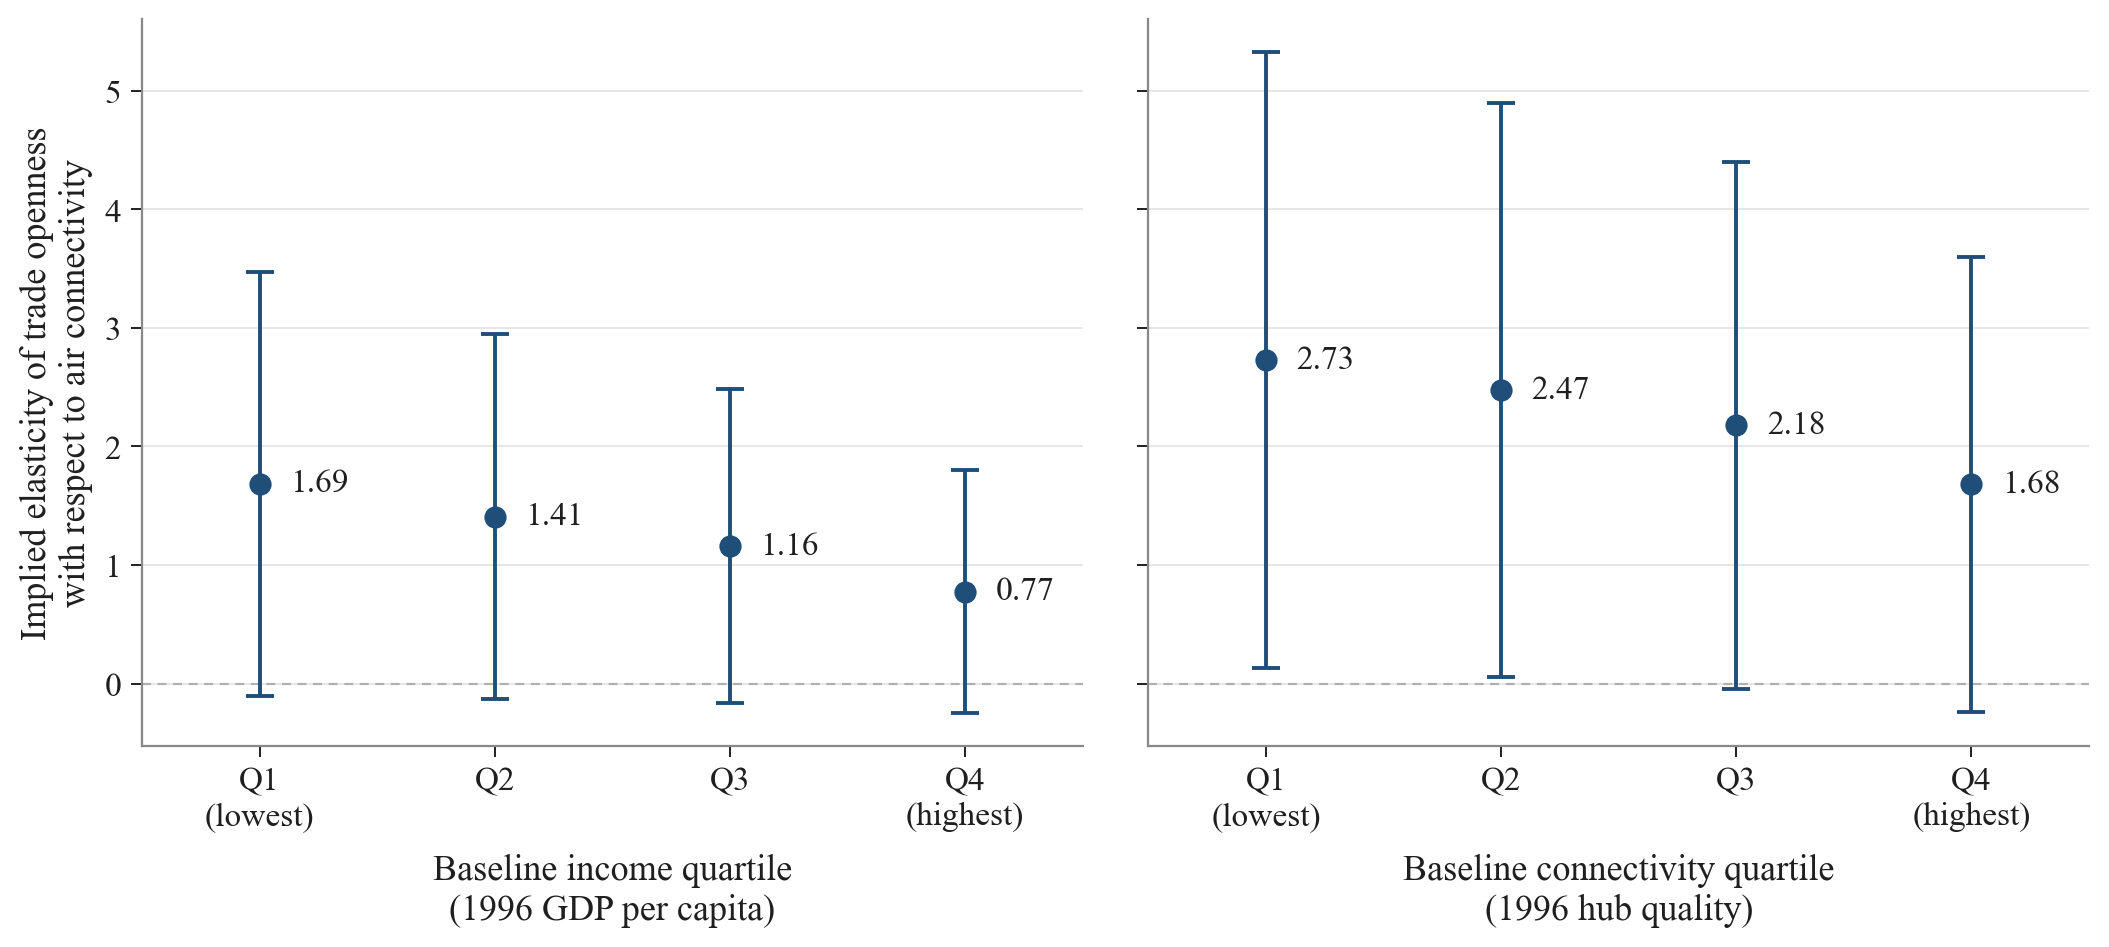
\includegraphics[width=0.95\linewidth]{GACI_hetero_quartile.png}
\caption{Implied elasticity of trade openness with respect to global aviation
connectivity, by baseline-income and baseline-connectivity quartile (Q1 = lowest;
95\% CIs).}
\label{fig:hetquartile}
\end{figure}

%=======================================================================
\subsection{Temporal heterogeneity}
\label{sec:temporal}
%=======================================================================
We also examine whether the effect has shifted over time by interacting
$\ln\mathrm{GACI}_{cwm}$ with a post-2010 indicator, 2010 being the midpoint
of the 1996--2023 sample (Table~\ref{tab:temporal}). Both the level and the
interaction are instrumented, by the tourism-heritage instrument and its
post-2010 interaction, and the joint first stage is of the same modest
strength as the interacted specifications above (KP $F=6.2$). Because the
instrument derives its power from the global tourism boom, its relevance is
inherently concentrated in the later period: a subsample diagnostic puts the
first-stage KP $F$ at $0.29$ before 2010 and $27.7$ afterwards, so the
pre-2010 level coefficients are not identified and we do not interpret them.
The informative estimand is the post-2010 shift, which is positive and
significant for volume and GDP: the impact is concentrated after 2010. This
concentration is not an artifact of the 2010 cutoff: re-estimating the model
at every split year from 2002 to 2013 leaves the pre-period first stage weak
throughout ($F<5$) and the post-2010 interaction for volume positive and
significant at the 1~percent level throughout ($0.24$--$0.54$). The timing
coincides with the era of low-cost long-haul and Gulf and Asian hub
expansion; these industry developments are plausible drivers of the shift,
but the design establishes only the temporal difference, not which post-2010
developments generate it.

\begin{table}[H]
\centering
\caption{Temporal heterogeneity: interaction with post-2010 (robust SE).}
\label{tab:temporal}
\begin{threeparttable}
\small
\begin{tabular}{lccc}
\toprule
 & Trade openness & Trade volume & GDP \\
\midrule
$\ln\mathrm{GACI}_{cwm}$ (pre-2010) & 1.247   & 0.496   & $-0.751$ \\
                        & (0.771) & (0.877) & (0.983) \\
$\times$ post-2010      & 0.012   & 0.377\sym{***} & 0.366\sym{***} \\
                        & (0.076) & (0.088) & (0.091) \\
\midrule
Country, Year FE        & Yes & Yes & Yes \\
First-stage KP $F$      & 6.22 & 6.22 & 6.22 \\
Observations            & 4{,}642 & 4{,}642 & 4{,}642 \\
\bottomrule
\end{tabular}
\begin{tablenotes}\small
\item Country and year FE; robust SE. Both endogenous terms are instrumented
by the tourism-heritage instrument and its post-2010 interaction; KP $F$ is
the joint Kleibergen--Paap statistic. A subsample diagnostic shows the
instrument is essentially irrelevant before 2010 (KP $F=0.29$) and strong
afterwards ($F=27.7$), so identification is concentrated in the post-2010
period.
\sym{***}~$p<0.01$.
\end{tablenotes}
\end{threeparttable}
\end{table}

%=======================================================================
\subsection{Mechanism: composition carries the openness effect}
\label{sec:mechanism}
\label{sec:mediation}
%=======================================================================
\textbf{Hypotheses~2} and \textbf{3} in Section~\ref{sec:framework} predict that if
connectivity works through high-value air cargo (\textbf{Hypothesis~2}) and
value-chain participation (\textbf{Hypothesis~3}), it should change the mix of trade,
and that this compositional change should carry the openness effect.
Table~\ref{tab:mechanism} tests both steps with two composition measures
built from BACI product-level data (Section~\ref{sec:data}): the log
ratio of intermediate to consumption goods, the value-chain margin, and
the log ratio of high to low unit-value trade, the air-freight margin.
Ratios net out shocks common to all of a country's trade, so they move
only when the trade mix moves.

The first step asks whether connectivity changes the trade mix, taking each composition ratio as the outcome. It does: a rise in hub quality shifts trade toward high value-to-weight goods (column (4): $1.71$, $p<0.05$), directly supporting \textbf{Hypothesis~2}, and the shift toward intermediate goods points the same way (column (2): $1.12$, s.e.\
$0.69$), consistent in sign with \textbf{Hypothesis~3} but not statistically significant at conventional levels. Connectivity does not raise all trade proportionally. It tilts the basket toward the goods that air transport serves.

The second step asks whether this compositional change carries the openness effect. The logic is a comparison across columns. If connectivity raised openness through some channel unrelated to composition, its coefficient should be unchanged when the composition ratios enter the openness regression as controls. If the effect operates through composition, the coefficient should fall toward zero while the ratios absorb it. The data choose the second reading. The connectivity coefficient falls from $1.27$ in column (1) to $1.09$ when the
intermediates ratio enters (column (3)) and to $1.00$, no longer statistically distinguishable from zero, when both ratios enter (column (6)). The composition ratios themselves are strong predictors of openness throughout: a trade basket tilted toward intermediates and high-value goods is a more open one (column (6): $0.173$, $p<0.01$ and $0.047$, $p<0.05$). The sample is identical in every column, so the decline of the connectivity coefficient reflects the controls, not the data. Taken together, the two steps are mutually consistent: connectivity re-composes trade toward air-served goods, and that re-composition absorbs the openness effect. Because the composition ratios are themselves equilibrium outcomes that other determinants of openness may also move, we read this pattern as supporting the proposed mechanisms rather than proving that they generate the effect (Section~\ref{sec:strategy}). Read against the hypotheses, both steps support \textbf{Hypothesis~2}: the trade mix shifts toward high value-to-weight goods, and that shift helps absorb the openness effect. \textbf{Hypothesis~3} receives qualified support: the shift toward intermediates
is imprecisely estimated in the first step, but the intermediates ratio is the single strongest absorber of the openness effect in the second, which is the pattern the value-chain channel requires.

\begin{table}[H]
\centering
\caption{Mechanism: connectivity, trade composition, and openness, 2SLS,
1996--2023.}
\label{tab:mechanism}
\begin{threeparttable}
\small
\begin{tabular}{lcccccc}
\toprule
 & (1) & (2) & (3) & (4) & (5) & (6) \\
Dependent variable: & Openness & $\ln\frac{\text{Interm.}}{\text{Consum.}}$ & Openness & $\ln\frac{\text{High VW}}{\text{Low VW}}$ & Openness & Openness \\
\midrule
$\ln\mathrm{GACI}_{cwm}$ & 1.268\sym{*} & 1.116 & 1.086\sym{*} & 1.714\sym{**} & 1.247\sym{*} & 0.996 \\
 & (0.656) & (0.693) & (0.638) & (0.753) & (0.668) & (0.649) \\
ln(Interm./Consum.) &  &  & 0.163\sym{***} &  &  & 0.173\sym{***} \\
 &  &  & (0.019) &  &  & (0.019) \\
ln(High/Low VW) &  &  &  &  & 0.012 & 0.047\sym{**} \\
 &  &  &  &  & (0.021) & (0.020) \\
\midrule
First-stage KP $F$ & 18.1 & 18.1 & 17.7 & 18.1 & 17.5 & 16.9 \\
Observations & 4{,}614 & 4{,}614 & 4{,}614 & 4{,}614 & 4{,}614 & 4{,}614 \\
\bottomrule
\end{tabular}
\begin{tablenotes}\small
\item Robust SE in parentheses. Openness is $\ln(\text{trade}/\text{GDP})$.
The composition ratios are built from BACI HS92 product-level data aggregated
to country-year values (exports plus imports): intermediate versus consumption
goods by BEC end-use, and high versus low unit-value trade split at the pooled
product median (USD/kg). All columns instrument $\ln\mathrm{GACI}_{cwm}$ with
the tourism-heritage instrument and include country and year FE and $\ln$
population, as in Table~\ref{tab:main}. Columns (2) and (4) take the ratios as
outcomes; columns (3), (5), and (6) add them as controls. Column (1) differs
marginally from Table~\ref{tab:main} because the sample requires nonmissing
composition ratios.
\sym{*}~$p<0.10$, \sym{**}~$p<0.05$, \sym{***}~$p<0.01$.
\end{tablenotes}
\end{threeparttable}
\end{table}

%=======================================================================
\subsection{Aggregate contribution of connectivity growth, 1996--2023}
\label{sec:aggregate}
%=======================================================================
The elasticity in Table~\ref{tab:main} on its own says little about how much trade is at stake. We therefore translate it into an aggregate magnitude. This serves two purposes: it expresses the estimate in units that matter for policy (dollars of trade and points of GDP), and it lets the contribution of two decades of global aviation connectivity growth be compared against the size of the world economy.

The calculation is a partial-equilibrium counterfactual. For each country we ask how much of its 2023 trade is attributable to that country's own 1996--2023 rise in hub quality, holding everything else fixed. Applying the openness elasticity, the attributable share is $1-\exp(-\beta\,\Delta\ln\mathrm{GACI}_{cwm,i})$ with $\beta=1.302$, so the implied gain is $\text{trade}_i\times\bigl(1-\exp(-\beta\,\Delta\ln\mathrm{GACI}_{cwm,i})\bigr)$. Summing across countries gives the world total.

On this basis, global aviation connectivity growth since 1996 is associated with about \textbf{\$7.8 trillion} of 2023 trade, roughly \textbf{17\%} of 2023 world trade (\$47 trillion) and \textbf{7.4\%} of 2023 world GDP, equivalently raising
world trade openness by about 7.4 percentage points of GDP. Two quantifications accompany this point estimate. First, applying the endpoints of the openness elasticity's 95 per cent confidence interval
($\beta\in[0.00,\,2.60]$) to the same calculation yields an attributable-trade range of \$0.03--12.4 trillion. The volume-channel counterpart ($\beta\in[0.78,\,3.82]$) is \$5.1--14.9 trillion. Across the three connectivity measures the point estimate spans \$6.8--7.8 trillion on the openness channel (Table~\ref{tab:contribution}), and country-level delta-method standard errors are reported in \ref{app:country}. Second, the instrument derives nearly all of its first-stage relevance from the post-2010 period (Section~\ref{sec:temporal}), whereas the counterfactual applies the elasticity to connectivity changes from 1996 onward, so the headline figure extrapolates a relationship identified from recent variation to the earlier part of the sample (Section~\ref{sec:discussion}). Figure~\ref{fig:continent} traces the implied openness gain by continent over time and shows these gains accrue most to the Middle East (Gulf hubs) and Asia (China), which pull away from the rest after 2005.

\begin{figure}[H]
\centering
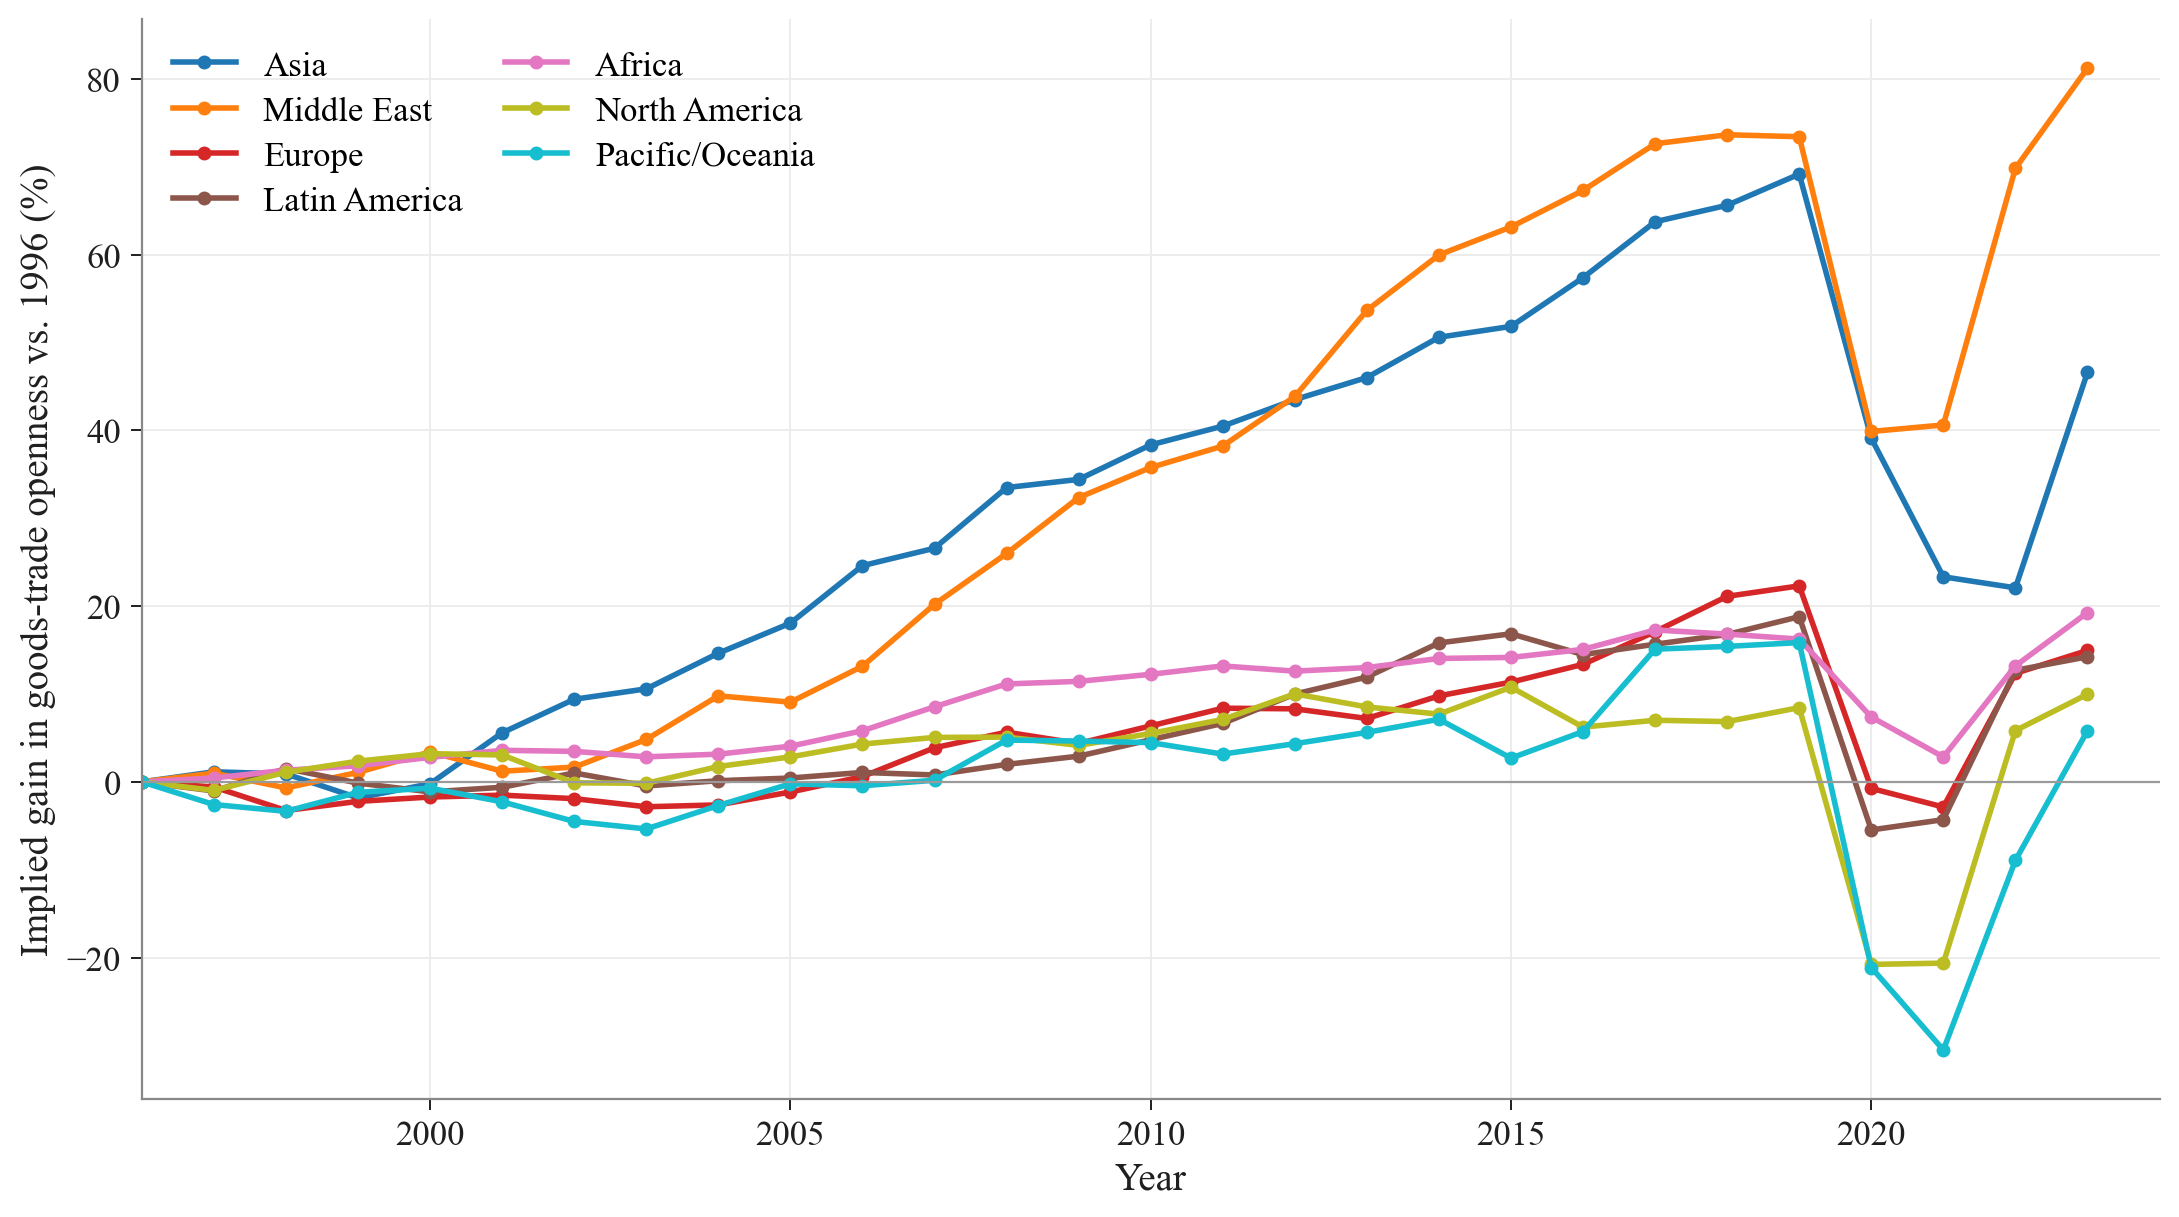
\includegraphics[width=0.85\linewidth]{GACI_continent_trend.png}
\caption{Implied gain in trade openness relative to 1996, by continent (openness
channel, $\beta=1.302$).}
\label{fig:continent}
\end{figure}

The headline figure uses hub quality ($\mathrm{GACI}_{cwm}$), but the magnitude is
not an artefact of that choice. Table~\ref{tab:contribution} repeats the
counterfactual for all three national connectivity aggregations (the
seat-capacity-weighted mean used in the headline, the single largest hub, and the sum
of airport indices), each with its own estimated elasticity. The implied trade contribution is strikingly stable: the openness channel attributes \$6.8--7.8 trillion of 2023 goods trade (14.5--16.5\% of
the world total), and the volume channel \$10.2--11.5 trillion (21.6--24.6\%),
regardless of measure. This stability is not mechanical, because the measures with
larger elasticities (hub quality) also display smaller log-changes over the period,
so the two offset. Applying the GDP-scale elasticity to GDP levels implies a further
\$9.8--13.2 trillion. We treat this as indicative only, since that elasticity is not
statistically distinguishable from zero.

Figure~\ref{fig:contribmap} disaggregates the world totals of Table~\ref{tab:contribution} to the country level, and three patterns stand out. First, the attributable gains are dominated by China, which alone accounts for roughly \$2.1 trillion of 2023 trade on the headline measure, followed by Korea, the United Arab Emirates, Japan, and Turkey. The map is the country-level counterpart of the continental divergence in Figure~\ref{fig:continent}. Second, the geography is stable across the three panels: the same countries shade in the same direction under all three connectivity measures, restating in map form the stability of the world totals. Third, the totals are net figures: 42 to 60 of the 184 countries, depending on the measure, experienced falling connectivity over the period, with Germany the largest implied loss on the headline measure, so the aggregate contribution accrues despite sizeable declines in some established hubs. Country-by-country implied effects, with delta-method standard errors, are tabulated in \ref{app:country}.

\begin{table}[H]
\centering
\caption{Aggregate contribution of aviation-connectivity growth, 1996--2023, under
three connectivity measures.}
\label{tab:contribution}
\begin{threeparttable}
\small
\begin{tabular}{lcccccc}
\toprule
 & \multicolumn{2}{c}{Trade, openness} & \multicolumn{2}{c}{Trade, volume}
 & \multicolumn{2}{c}{GDP, scale} \\
\cmidrule(lr){2-3}\cmidrule(lr){4-5}\cmidrule(lr){6-7}
Measure & $\beta_{\text{int}}$ & \$tn\,(\%\,wT) & $\beta_{\text{vol}}$ & \$tn\,(\%\,wT)
 & $\beta_{\text{GDP}}$ & \$tn\,(\%\,Y) \\
\midrule
$\mathrm{GACI}_{cwm}$ (headline) & 1.302 & 7.8\ (16.5) & 2.303 & 11.5\ (24.6) & 1.001 & 13.2\ (12.6) \\
$\mathrm{GACI}_{max}$ & 0.966 & 6.8\ (14.5) & 1.709 & 10.2\ (21.6) & 0.743 & \phantom{0}9.8\ (\phantom{0}9.4) \\
$\mathrm{GACI}_{sum}$ & 0.659 & 7.5\ (16.0) & 1.166 & 10.5\ (22.4) & 0.507 & 13.0\ (12.5) \\
\bottomrule
\end{tabular}
\begin{tablenotes}\small
\item Each dollar cell is the world sum of country-level attributable gains,
$\sum_i \text{level}_i(2023)\times[1-\exp(-\beta\,\Delta\ln\mathrm{GACI}_i)]$, where
$\beta$ is the corresponding 2SLS elasticity and $\Delta\ln\mathrm{GACI}_i$ is the
country's 1996--2023 change in that measure. ``Openness'' applies the
trade-openness elasticity to goods-trade levels (headline); ``volume'' the
trade-volume elasticity (an upper bound folding in the GDP-scale channel);
``GDP, scale'' the GDP elasticity to GDP levels. World bases are 2023 goods
trade (\$46.9~trillion) and GDP (\$104.6~trillion); \%\,wT and \%\,Y are the
corresponding world shares. Volume elasticities are significant at 1\% for all
three measures, openness at 5\% (max, cwm) and 10\% (sum); GDP elasticities are
not significant, so the GDP columns are indicative only.
\end{tablenotes}
\end{threeparttable}
\end{table}

\begin{figure}[H]
\centering
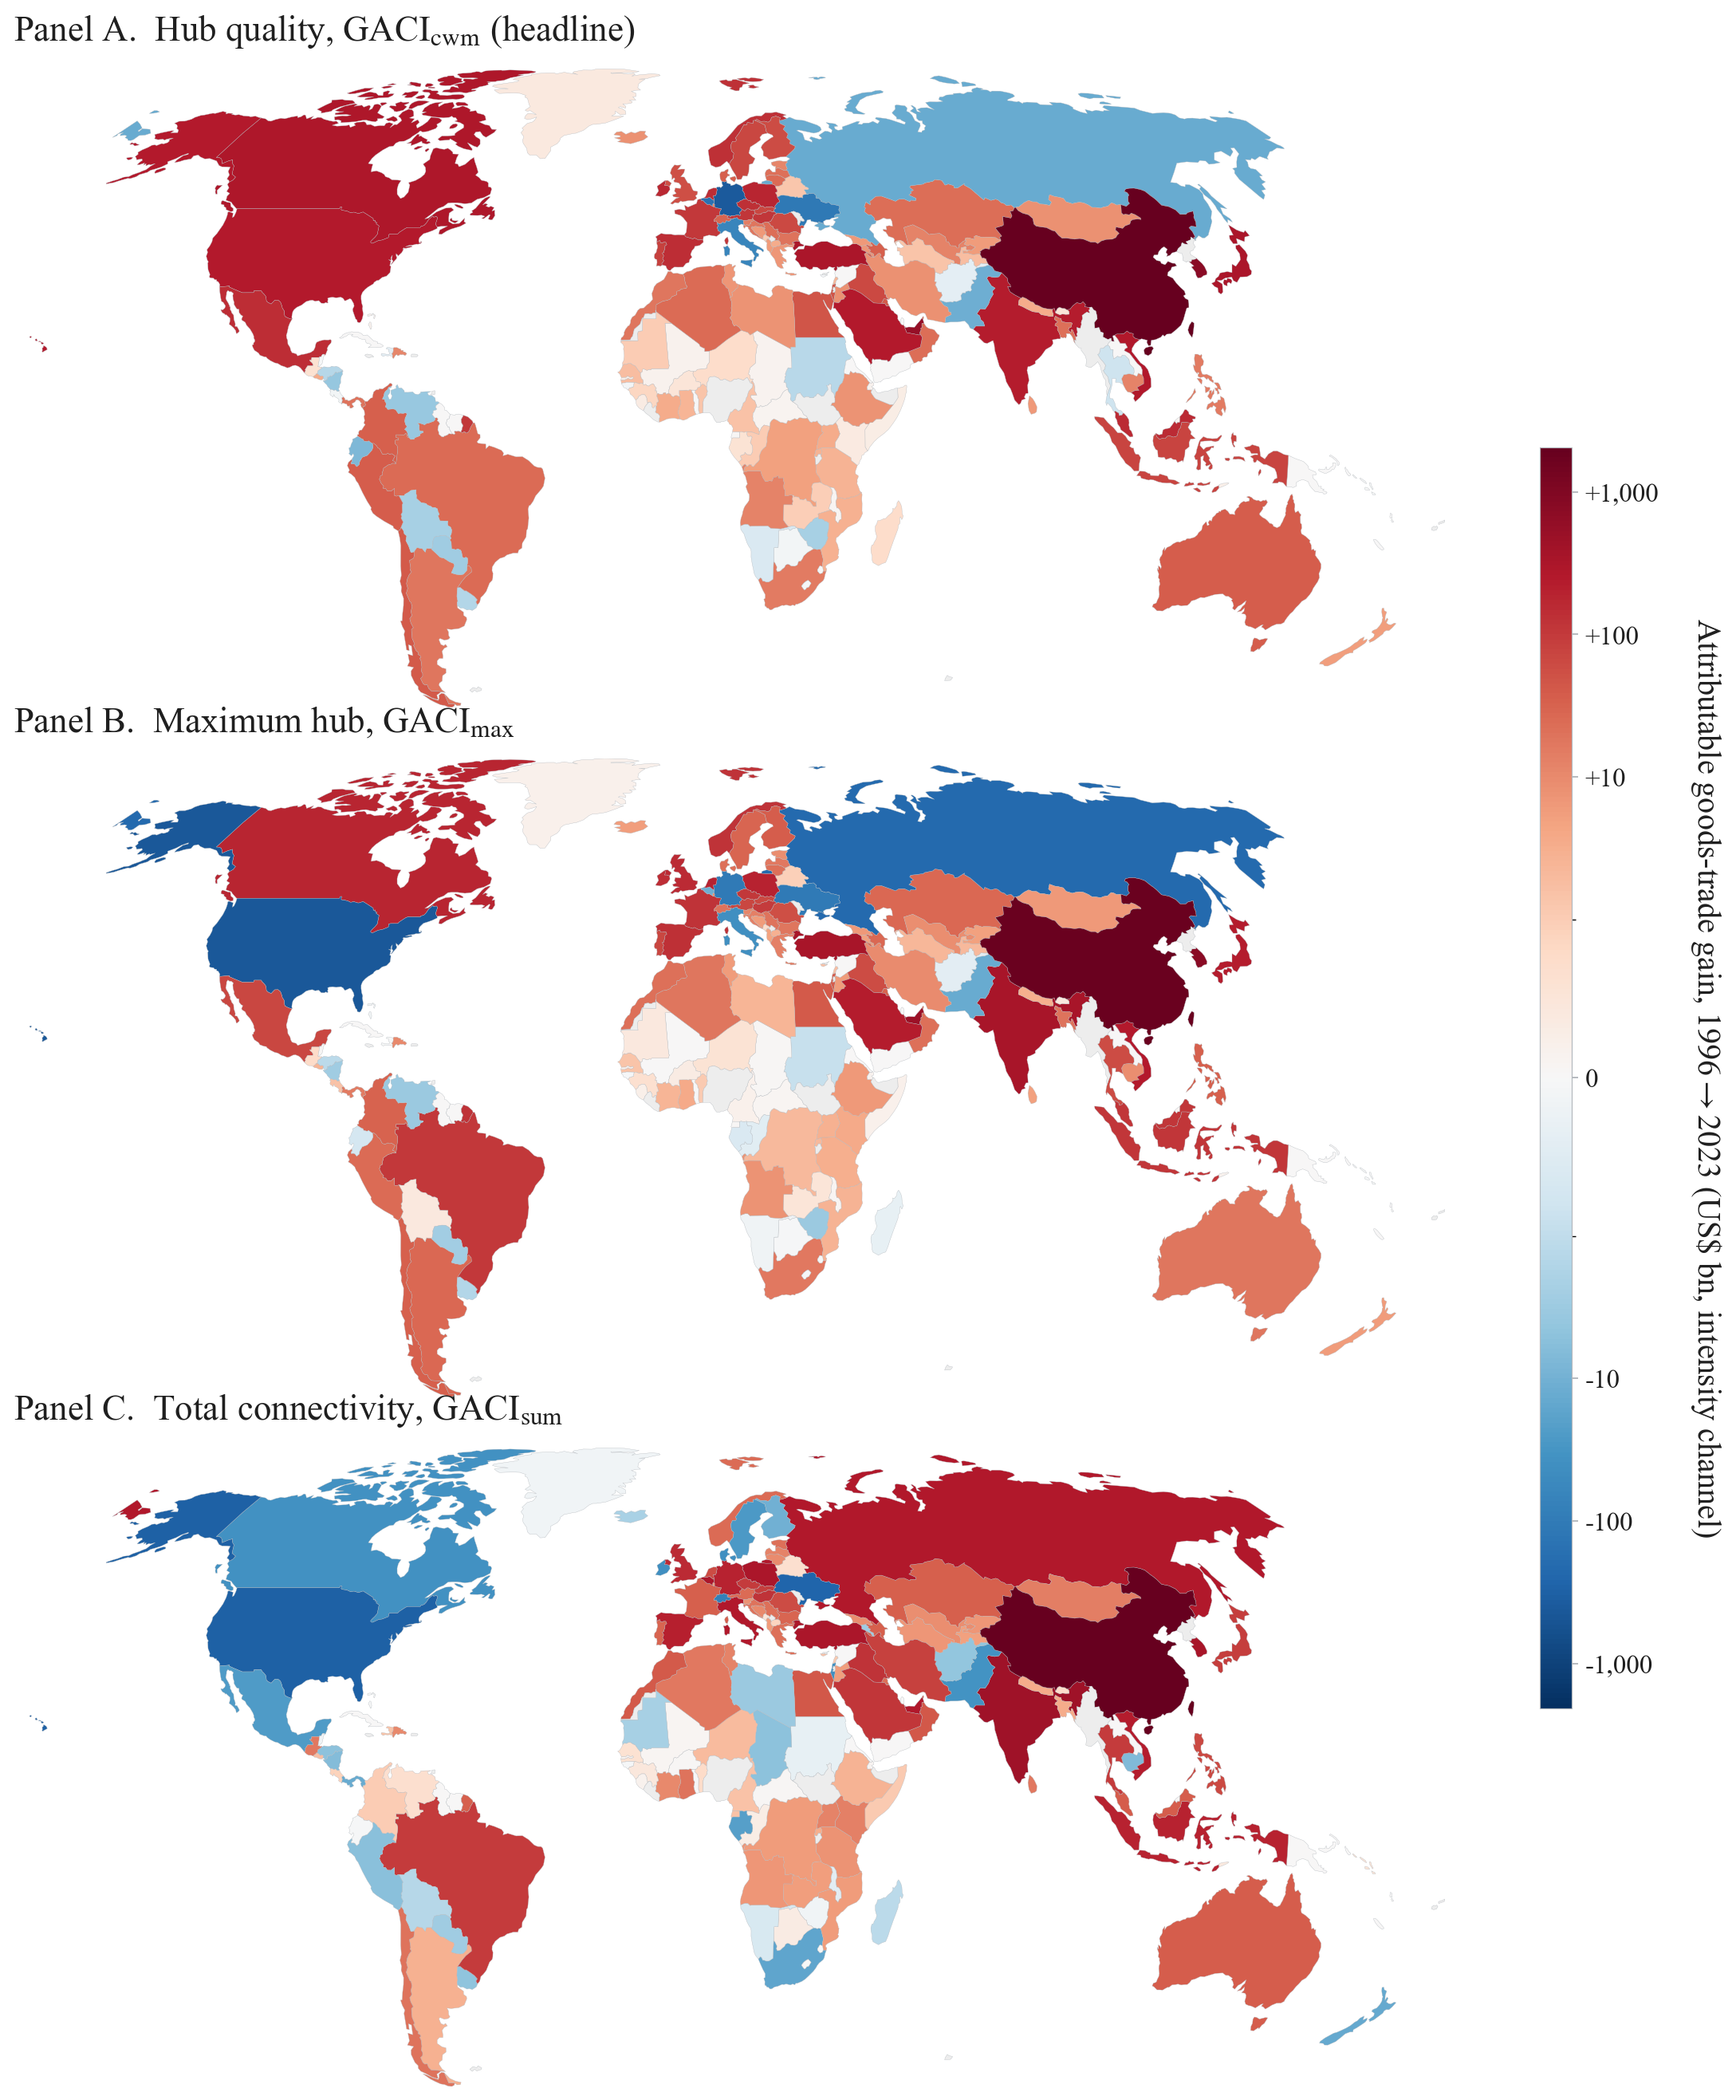
\includegraphics[width=0.85\linewidth]{GACI_contrib_trade_3panel.png}
\caption{Country-level contribution of aviation-connectivity growth to goods trade,
1996--2023 (openness channel), under the three connectivity measures. Red denotes
positive attributable trade (connectivity rose), blue negative (connectivity fell on
that measure), and grey is outside the sample. Gains are dominated by China, India,
and emerging Asia; a sizeable minority of countries (42--60 of 184, depending on the
measure) saw connectivity fall over the period, so the world totals in
Table~\ref{tab:contribution} are net of these losses.}
\label{fig:contribmap}
\end{figure}

%=======================================================================
\subsection{Connectivity-collapse shocks}
%=======================================================================
If the estimated relationship operates symmetrically, the same logic applies in reverse: an abrupt collapse should subtract the trade that expansion built. Symmetry between expansion and contraction is an assumption of this exercise rather than an established result (Section~\ref{sec:discussion}). We apply the counterfactual to the COVID-19 collapse (2019 to 2020) for all three measures, keeping hub quality ($\mathrm{GACI}_{cwm}$) as the headline for consistency with the rest of the paper. 

Connectivity fell in 154 of 175 countries on the hub-quality measure (median $\Delta\ln\mathrm{GACI}_{cwm}=-0.073$), implying a one-year goods-trade disruption of about \$7.5 trillion, roughly 20\% of 2019 world trade; the maximum-hub measure implies \$6.7 trillion (18\%), and total connectivity \$1.8 trillion (4.8\%). The wide spread between the hub-quality and sum-based figures compounds two differences: the sum-based figure carries both the smallest openness elasticity ($0.659$ against $1.302$ for hub quality) and the smallest measured collapse, because summed connectivity is dominated by the count of airports with any scheduled service, which contracted far less in 2020 than capacity-weighted network position did. The corresponding GDP contraction ranges from \$2.5 trillion (total connectivity) to \$13.2 trillion (hub quality), about 3 to 15\% of 2019 world GDP, though it rests on the imprecise GDP elasticities and is only indicative. Two cautions attach to these magnitudes. First, the elasticities are long-run cross-country estimates, so applying them to a single year overstates the short-run response: the figures are best read as a range of estimates, with the hub-quality figure toward the upper end and the sum-based figure toward the lower end, rather than as hard bounds. Second, in 2020 connectivity and trade fell together under a common shock (pandemic demand and lockdowns), so the exercise attributes to connectivity a contraction that has other causes as well; the implied disruption should therefore not be interpreted as the causal trade loss from reduced connectivity alone. 

With those caveats, the direction is consistent across all three measures: an abrupt connectivity collapse coincides with a large trade contraction, concentrated in the major gateway hubs that had gained the most on the way up. Figure~\ref{fig:shock} maps the effect country by country for each measure. The largest implied losses fall on the United States and the gateway economies of Europe and East Asia (Germany, Hong Kong, Korea, Japan, Singapore, the Netherlands), while the loss itself is nearly universal across the map. The scattered gains in Panel~C are mechanical rather than economic: total connectivity sums over all airports with scheduled service, and 36 of the 175 countries observed in both years saw their summed index rise in 2020, so the counterfactual assigns them a gain even as global connectivity collapsed.

\begin{figure}[H]
\centering
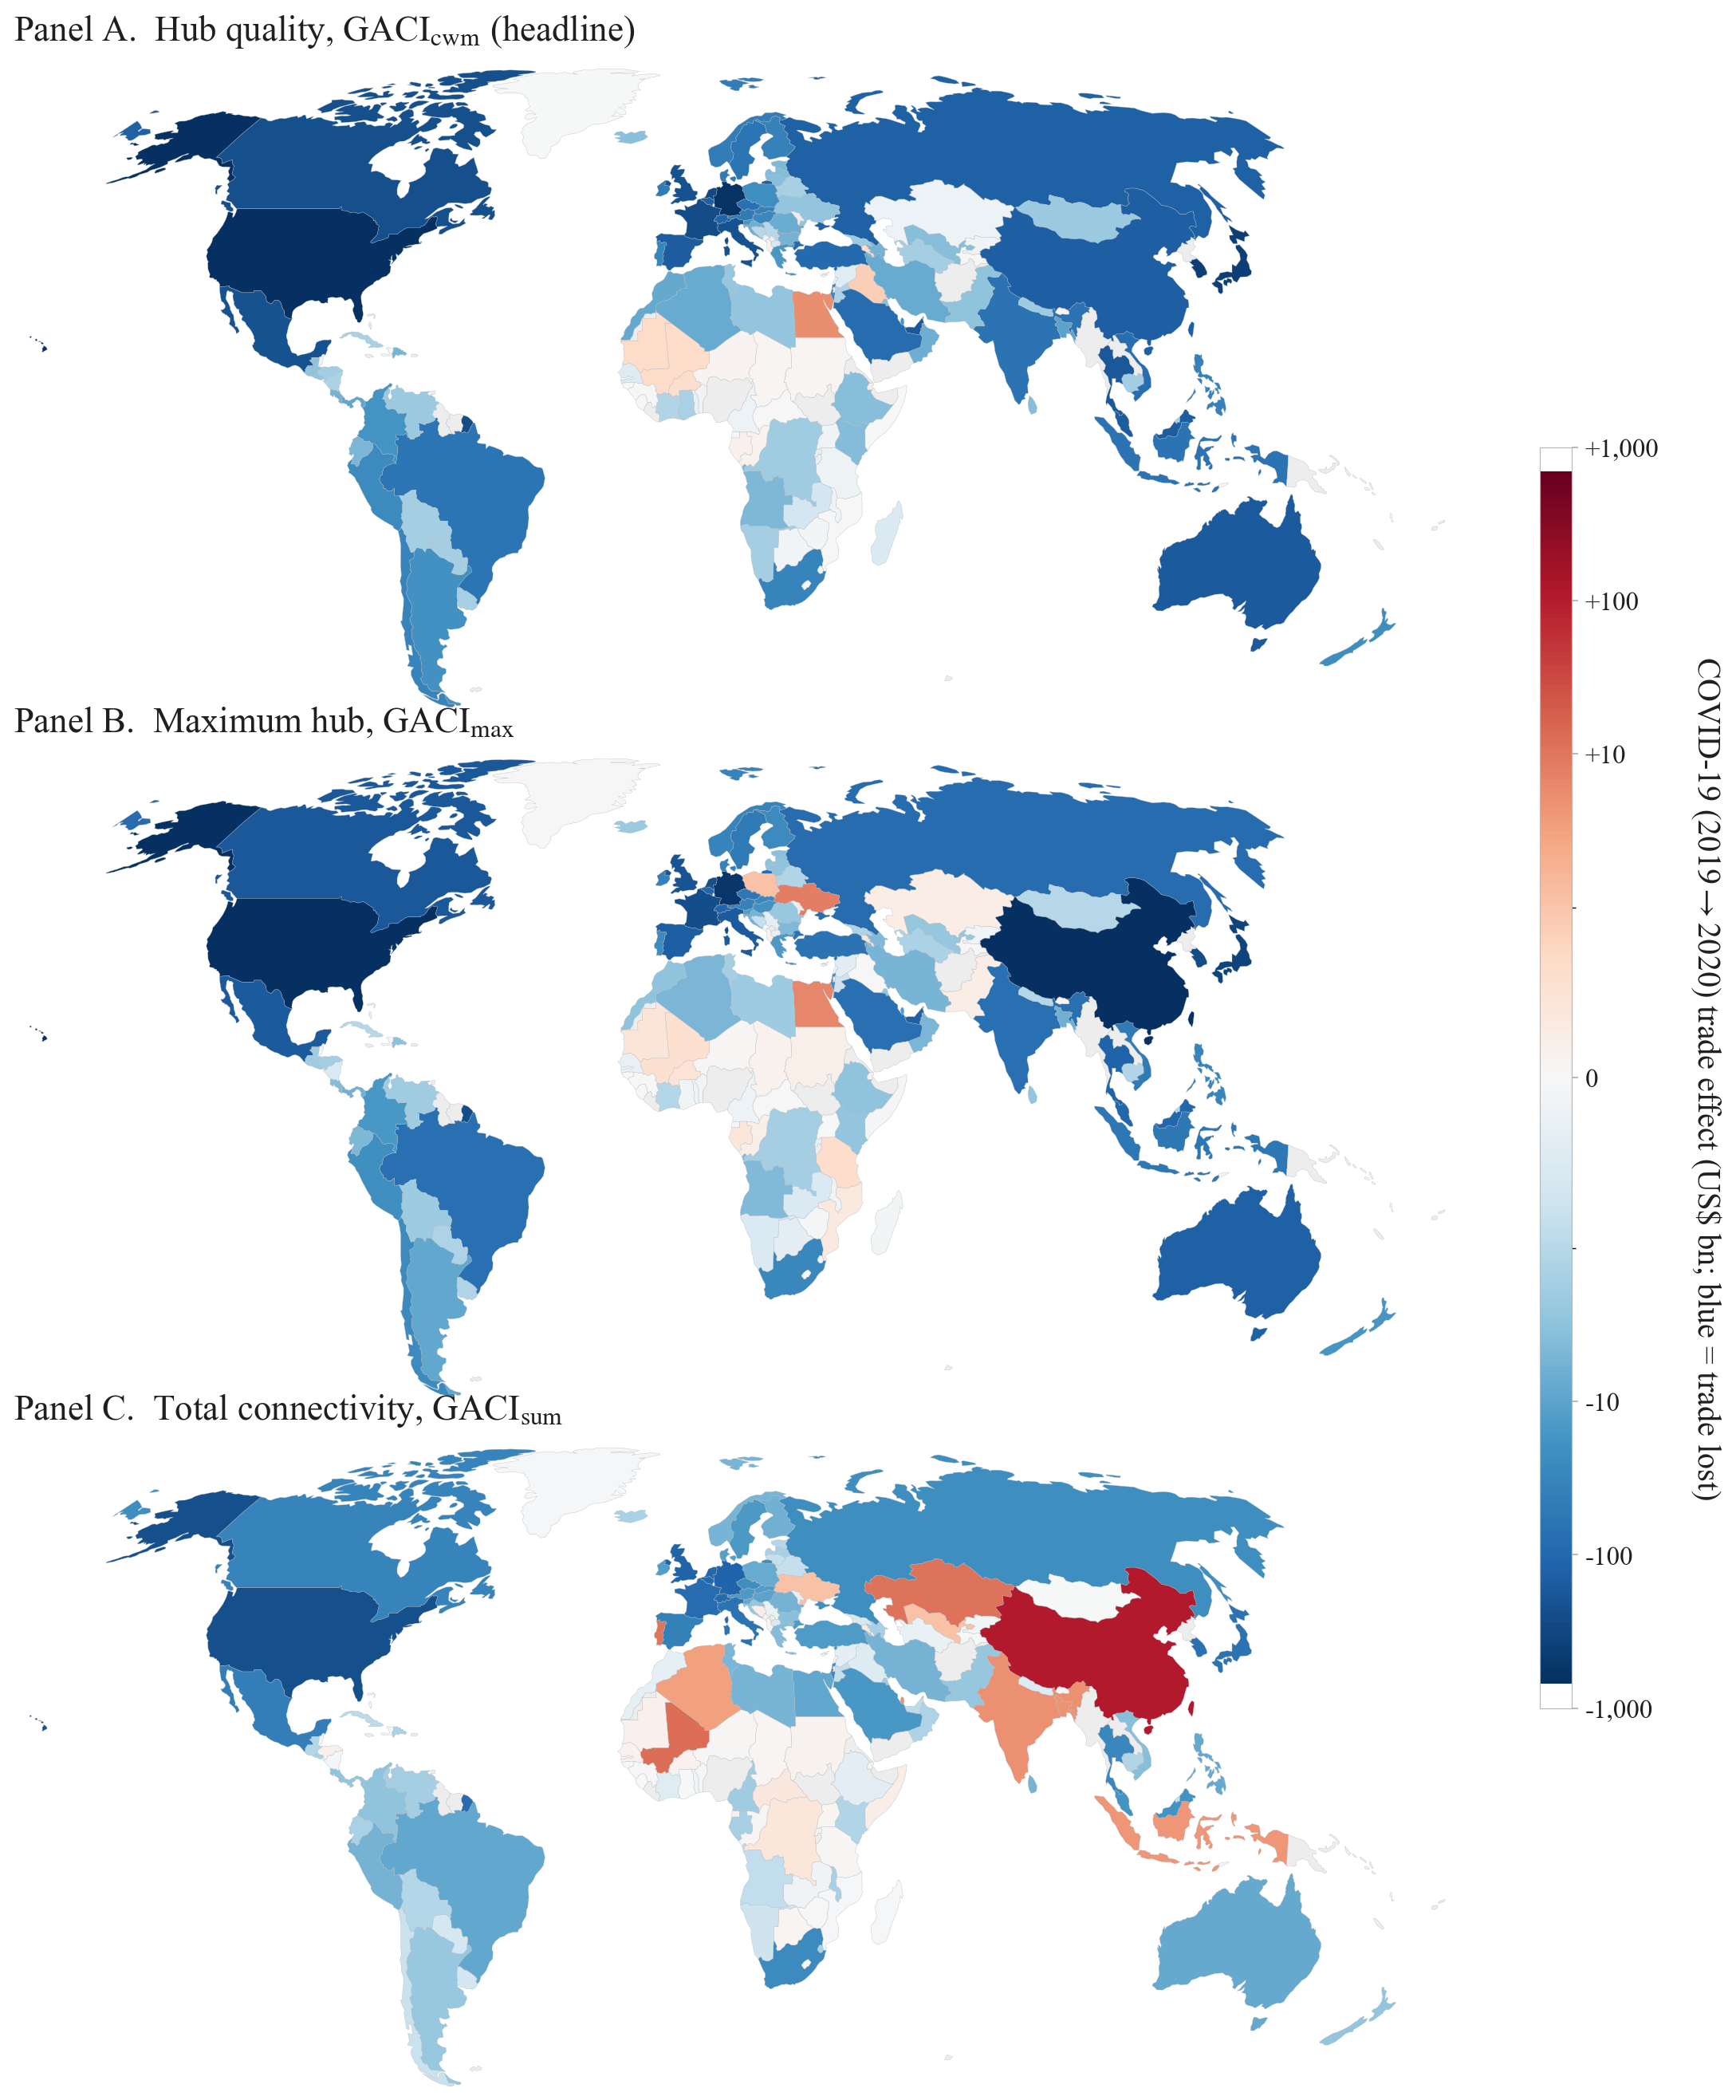
\includegraphics[width=0.85\linewidth]{GACI_covid_shock_3panel.png}
\caption{COVID-19 (2019 to 2020): implied country-level goods-trade effect of the
aviation-connectivity collapse, under the three connectivity measures. Blue denotes
trade lost, red trade gained, and grey is outside the sample. The loss is broad and
concentrated in major gateway hubs; under total connectivity (Panel C) a few
countries register mechanical gains because their summed index rose over the year.}
\label{fig:shock}
\end{figure}

%=======================================================================
\subsection{Synthesis: the hypotheses revisited}
\label{sec:synthesis}
%=======================================================================
The results map onto the three hypotheses of Section~\ref{sec:framework} as follows. \textbf{Hypothesis~1}, that higher aviation connectivity increases merchandise trade, is supported: instrumented hub quality raises goods-trade
volume with an elasticity of $2.30$ and trade openness with an elasticity of $1.30$ (Table~\ref{tab:main}), the pattern holds across all three aggregations of connectivity, and the estimates survive the validity checks
of \ref{sec:robust}. \textbf{Hypothesis~2}, that connectivity raises the share of high value-to-weight and time-sensitive goods, is supported: connectivity shifts the trade mix toward high unit-value goods (Table~\ref{tab:mechanism}, column (4)), and this margin helps carry the openness effect once entered as a control. \textbf{Hypothesis~3}, that connectivity raises intermediate-goods trade relative to final consumption goods, receives partial support: the estimated shift toward intermediates is positive but not statistically significant at conventional levels, yet the intermediates ratio is the strongest single absorber of the openness effect, a pattern consistent with, though not conclusive for, the value-chain channel.

Read jointly, the three verdicts tell one story rather than three. The level effect that \textbf{Hypothesis~1} establishes is not spread uniformly across the trade basket. It is carried by precisely the composition margins that \textbf{Hypotheses~2} and \textbf{3} single out, since the connectivity coefficient on openness falls to statistical insignificance once the two composition ratios are controlled for. This also disciplines the interpretation of the transaction-cost channel behind \textbf{Hypothesis~1}: a pure reduction in generalised trade frictions would raise trade across all product types and leave the mix unchanged, whereas the data show the openness gain travelling through
air-served goods. Aviation connectivity raises merchandise trade, in other words, by enabling the kinds of trade that air transport makes feasible, not by lifting all trade alike.

Taken together, these results carry four messages. First, global aviation connectivity is a causal driver of trade integration, and it operates primarily on the openness margin: better-connected countries trade more relative to the size of their economies, not merely because they are larger. Second, the effect works through composition: connectivity tilts the trade mix toward high value-to-weight goods and, with less precision, intermediate goods, and this shift carries the openness effect. Third, the returns are unevenly shared and are largest for poorer and less-connected economies, so aviation acts as a convergence lever. Fourth, because connectivity builds trade on the way up, abrupt collapses subtract it on the way down, as the COVID-19 episode shows. The policy implication is direct: airport and route investment and air-service liberalisation are concrete levers for trade integration, with the highest marginal returns in under-connected economies.

%=======================================================================
\section{Discussion}
\label{sec:discussion}
%=======================================================================
The central finding of this study is that global air connectivity is
associated with deeper trade integration, not merely with larger economies.
The 2SLS estimate for the headline hub-quality measure implies an elasticity
of trade openness of $1.30$, and the positive relationship is preserved when
connectivity is represented by the country's largest hub or by total
airport-system connectivity. By contrast, the estimated GDP elasticity is
positive but not statistically significant. The empirically better-supported
component of the trade-volume response is therefore the openness margin:
countries with stronger positions in the global air network trade more
relative to the size of their economies. The exact decomposition of the
trade-volume coefficient into openness and GDP components follows from the
accounting identity linking the three outcomes; its substantive value lies
not in the arithmetic itself, but in showing which component is statistically
supported. More broadly, the result supports an interpretation of aviation
connectivity as economic accessibility. What matters is not only the amount
of aviation activity within a country, but how effectively its airports
connect firms, suppliers, customers, and production partners to the wider
global network.

The product-level results help explain why this relationship may arise, while
also indicating where the evidence is stronger and weaker. Connectivity
significantly shifts the trade mix toward higher unit-value goods, a proxy
for products with high value-to-weight ratios for which rapid transport,
reliable coordination, and face-to-face interaction are particularly
valuable. This finding helps reconcile the importance of passenger-based
aviation connectivity with the fact that most international freight tonnage
moves by sea: aviation can facilitate trade by transporting time-sensitive
goods in passenger-aircraft belly capacity and by moving the people,
information, samples, and urgent inputs that support transactions regardless
of the mode used for the final shipment. Evidence for the global-value-chain
channel is more tentative. The estimated shift toward intermediate goods is
positive but not statistically significant at conventional levels. In
addition, the reduction in the GACI coefficient after the composition
measures are introduced should be interpreted as a descriptive decomposition
rather than formal causal mediation, because trade composition is itself an
outcome of connectivity. The results are therefore consistent with, but do
not conclusively establish, a compositional mechanism.

The heterogeneity results suggest that the returns to additional connectivity
are unevenly distributed. The most consistent gradients are observed with
respect to baseline income and baseline connectivity: poorer and initially
less-connected economies appear to obtain larger trade effects from
improvements in network position. This pattern is economically plausible
because the marginal value of accessibility may be greater where
international market access is otherwise limited and where the country has
not yet reached a mature hub position. It also gives the findings a
development-policy dimension, suggesting that improvements in effective
air-network access may yield larger trade-integration benefits in
under-connected economies than in already established global hubs. These
estimates, however, are less precisely identified than the average effect.
The interacted specifications have modest first-stage statistics, and the
gradients should therefore be read as suggestive rather than as precise
country-specific treatment effects. Accordingly, policy prioritisation should
be based on the robust average relationship and the broad income and
baseline-connectivity patterns, rather than on overly precise rankings of
countries by expected marginal returns.

These findings imply that aviation connectivity belongs alongside ports,
surface infrastructure, and trade agreements in the broader policy toolkit
for economic integration. Airport investment, route development, and
air-service liberalisation may contribute to trade integration when they
improve a country's effective position in the global network, particularly
its access to important destinations and onward connections. Because GACI
captures direct links, indirect accessibility, transfer centrality, and the
importance of connected airports, an intervention should not be judged solely
by the number of routes or seats that it adds. A route that strengthens
access to a major connecting hub may have a different economic value from an
otherwise similar increase in capacity to a peripheral destination. The
results therefore support evaluating aviation projects and liberalisation
policies in terms of system-wide accessibility and spillovers rather than
local traffic alone. Given the stronger evidence for high-value trade,
aviation policy may also have an industrial-policy dimension. At the same
time, the treatment identified here is a continuous change in composite
network position, not the opening of one specific route. Translating the
estimated elasticity into the benefit of an individual project or agreement
requires an additional model of how that intervention changes GACI.

The aggregate counterfactual conveys the potentially large economic scale of
the estimated relationship, but it should be interpreted as an attribution
rather than a literal accounting of trade created by aviation. Applying the
openness elasticity to observed connectivity growth attributes approximately
\$7.8 trillion of 2023 goods trade to changes in hub quality since 1996, and
comparable magnitudes arise under alternative national GACI aggregations.
This stability is informative, yet the calculation remains partial
equilibrium: it holds constant the changes in prices, production locations,
trading partners, modal substitution, airline responses, and network
reconfiguration that would accompany a different global aviation system. It
also applies a common pooled elasticity across countries even though the
heterogeneity results suggest that effects may vary with baseline income and
connectivity. Most importantly, the tourism-heritage instrument derives
nearly all of its first-stage relevance from the post-2010 period, whereas
the counterfactual applies the estimated elasticity to connectivity changes
beginning in 1996. The headline magnitude therefore extrapolates a
relationship identified primarily from recent variation to the earlier
portion of the sample. A post-2010 counterfactual would provide a useful
identification-aligned benchmark.

The COVID-19 exercise offers a complementary resilience perspective but does
not independently identify the causal effect of the pandemic or demonstrate
symmetry between network expansion and contraction. It applies the long-run
cross-country elasticity to the abrupt decline in connectivity between 2019
and 2020, producing implied trade disruption of \$1.8--7.5 trillion across
the three connectivity measures. The calculation is informative as an illustration of
the trade exposure associated with a sudden loss of network access,
especially in gateway economies. Nevertheless, a long-run elasticity may
overstate adjustment within a single year, and COVID-19 simultaneously
reduced aviation connectivity and trade through travel restrictions,
production disruptions, and demand shocks. The implied losses therefore
cannot be attributed to connectivity deterioration alone. The broader
resilience implication is more defensible: unlike physically persistent
infrastructure, aviation accessibility can contract rapidly even when
airports remain in place because it depends on airlines continuing to operate
routes and capacity. Preserving strategically important network access during
disruptions may consequently have value beyond passenger mobility.

The causal interpretation is strengthened by the similarity of the results
across alternative GACI aggregations, control specifications, falsification
exercises, and instrument designs. In particular, the independent
air/sea-distance instrument produces a trade-volume elasticity close to that
obtained from the tourism-heritage instrument, reducing concern that the
headline estimate is an artefact of a single identification strategy. These
checks do not, however, prove the exclusion restriction. The interpretation
remains conditional on the assumption that differential heritage exposure to
the global tourism cycle affects merchandise trade through air connectivity
rather than through an unobserved time-varying channel. Moreover, the IV
estimate is most directly informative about connectivity changes induced by
this source of variation; applying it to substantially different
policy-induced changes assumes that the relevant marginal effect is
comparable. The concentration of identifying power after 2010 further limits
claims about earlier aviation regimes.

Several future directions follow directly. First, bilateral product-level
trade could be analysed within a gravity framework, allowing changes in
aviation connectivity to be linked to specific origin--destination trade
relationships and distinguishing market-access effects from changes in
country-level totals. Embedding these relationships in a general-equilibrium
trade model would permit prices, production, partner choice, and modal
substitution to adjust endogenously. Such a framework would also allow the
cross-border dimension of connectivity to be studied directly: because the
index is a network measure, improvements at one hub can benefit neighbouring
economies, so the economic gains from connectivity need not accrue in the
country where the aviation activity, and its local externalities, are
located. Second, the internal composition of
GACI warrants separate investigation. The present analysis estimates the
effect of a composite index built from degree, flow betweenness, closeness,
eigenvector centrality, and regional importance, but it does not identify
which network dimension is most consequential for trade. Distinguishing the
roles of direct connectivity, transfer-hub function, global topological
accessibility, connections to influential hubs, and regional network strength
would provide more actionable policy guidance, although doing so would
require additional identification strategies and careful treatment of the
strong correlations among components. Third, combining passenger-network
measures with dedicated air-cargo capacity and business-travel data could
separate the belly-cargo, face-to-face, and coordination channels more
directly. Finally, post-2010 mechanism estimates, temporally aligned
counterfactuals, and research designs that distinguish gradual expansion from
abrupt contraction would clarify how stable the estimated relationship is
across aviation regimes and shock types. Together, these extensions would
translate the study's central finding, that global air connectivity is an
economically meaningful dimension of trade accessibility, into more precise
guidance on which forms of connectivity matter, for whom, and under what
conditions.

%=======================================================================
\section{Conclusion}
\label{sec:conclusion}
%=======================================================================
The evidence in this paper indicates that air connectivity is a causal driver
of goods-trade integration. Instrumenting a
continuous, network-based connectivity index with a heritage--tourism
shift-share instrument, we estimate a goods-volume elasticity of $2.30$ (an
openness elasticity of $1.30$ plus a GDP-scale elasticity of $1.00$) that
survives over-identification tests, an independent air/sea-distance instrument,
an alternative connectivity measure, and a cultural-heritage falsification.
Product-level data show how the effect works: connectivity tilts the trade mix
toward high value-to-weight and, more tentatively, intermediate goods, and
this compositional shift carries the openness effect. The payoff is largest for poorer and
under-connected economies, and two decades of connectivity growth account for
on the order of \$7.8 trillion of 2023 goods trade. The policy implications are
direct: airport and route investment and air-service liberalisation are
concrete, spillover-aware levers for trade and income, with the largest returns
in under-connected economies. Limitations include the partial-equilibrium nature of
the aggregation, the post-2010 concentration of identifying variation, and
weaker first stages in the heterogeneity splits. The estimates are
accordingly most informative about connectivity changes of the kind the
instruments induce, in the recent aviation era; extending the design to
bilateral flows within a gravity structure, and embedding the elasticities in
a general-equilibrium trade model in which prices, partners, and modal choice
adjust, are the natural next steps.

%=======================================================================
\appendix
%=======================================================================
\section{Instrument validity and robustness}
\label{sec:robust}
%=======================================================================
Section~\ref{sec:data} stated the exclusion restriction, that heritage-driven
tourism demand affects goods trade only through air connectivity, and the
design choices that narrow the space of violations before any testing: the
merchandise outcome removes the services channel by construction, the share
is restricted to natural and mixed sites, and country fixed effects absorb
every time-invariant characteristic, geography, coastline, or colonial
history, through which heritage endowments could otherwise matter. These
choices narrow the space of violations but do not eliminate it: excluding
services and tourism from the outcome removes the mechanical channel from
tourist spending, not every indirect effect of tourism demand on merchandise
trade, which could still operate through income, prices, or the real
exchange rate. This
section probes what remains, in three steps: sensitivity to controls, formal
over-identification and falsification tests, and an independent instrument.

\paragraph{Sensitivity to controls.} A first, simple check is whether the
estimate depends on what else is in the regression \citep[cf.][]{Frankel_1999}.
Because country fixed effects absorb all time-invariant controls, the feasible
time-varying candidates are population and income. Table~\ref{tab:controls}
re-estimates the headline openness regression under five control sets. The
estimate barely moves: $1.66$ with no controls, $1.30$ with population (the
baseline), $1.71$ with GDP, $1.64$ with both, and $1.43$ with population and
GDP per capita, always significant at the 5 per cent level, with the first
stage strong throughout (KP $F=15.1$--$20.9$). Note that GDP is itself an
outcome of connectivity (Table~\ref{tab:main}), so conditioning on it
over-controls; that the openness effect survives even this conservative check
is reassuring.

\begin{table}[H]
\centering
\caption{Sensitivity to controls: 2SLS effect of connectivity on trade
openness under alternative control sets.}
\label{tab:controls}
\begin{threeparttable}
\small
\begin{tabular}{lccccc}
\toprule
 & (1) & (2) & (3) & (4) & (5) \\
Controls: & None & $\ln$ pop.\ & $\ln$ GDP & $\ln$ pop.\ $+$ & $\ln$ pop.\ $+$ \\
 & & (baseline) & & $\ln$ GDP & $\ln$ GDP p.c.\ \\
\midrule
$\ln\mathrm{GACI}_{cwm}$ & 1.663\sym{**} & 1.302\sym{**} & 1.706\sym{**} & 1.642\sym{**} & 1.430\sym{**} \\
 & (0.775) & (0.662) & (0.688) & (0.686) & (0.704) \\
\midrule
First-stage KP $F$ & 15.1 & 18.0 & 19.1 & 18.9 & 20.9 \\
Observations & 4{,}642 & 4{,}642 & 4{,}642 & 4{,}642 & 4{,}642 \\
\bottomrule
\end{tabular}
\begin{tablenotes}\small
\item Robust SE in parentheses. Dependent variable: trade openness,
$\ln(\text{trade}/\text{GDP})$. All columns instrument $\ln\mathrm{GACI}_{cwm}$
with the tourism-heritage instrument and include country and year FE; only the
time-varying controls differ. Column (2) is the baseline specification of
Table~\ref{tab:main}. GDP is itself an outcome of connectivity, so columns
(3)--(5) over-control; the stability of the estimate is a conservative check.
\sym{**}~$p<0.05$.
\end{tablenotes}
\end{threeparttable}
\end{table}

Table~\ref{tab:robust} collects the formal tests of the identifying assumption.

\paragraph{(A) Over-identification with natural and mixed heritage.} Entering
natural and mixed heritage as two separate instruments over-identifies
the single endogenous regressor and licenses a Hansen $J$ test. The two
instruments are not statistically inconsistent: the Hansen $J$ is far from
rejection for every outcome, and the volume
elasticity is essentially unchanged ($2.18$, $p<0.01$). The first stage is
weaker than in the baseline model (KP $F=8.5$), suggesting weaker first-stage
identification, so we read this over-identified estimate as corroborating the
baseline rather than replacing it.

\paragraph{(B) Falsification: adding cultural heritage.} Cultural heritage
co-moves with development and historic urban and manufacturing centres, so it
is a plausible exclusion-violator. Adding it as a third instrument moves the
Hansen $J$ to rejection for the volume outcome ($p=0.004$) and collapses the
point estimate. The data thus reject cultural heritage as a valid
instrument, exactly the discriminating result that supports restricting the
instrument to natural and mixed endowments.

\paragraph{(C) Independent air/sea-distance instrument.} As an identification
path that shares no variation with tourism or heritage, we construct a
Frankel--Romer/Feyrer-type predicted air-linkage instrument from geography and
the CERDI sea-distance database
\citep{Frankel_1999,Feyrer_2019,Bertoli_2016}. The construction follows the
logic of \citet{Feyrer_2019}: a country's distances to world markets are
fixed by geography, but the relative economic importance of air over sea
transport has risen as global aviation expanded. The instrument interacts
each country's predetermined baseline (1996) air market access, the sum of
foreign populations weighted by inverse great-circle distance, with a global
aviation-intensity index built from world scheduled seat capacity, common to
all countries; sea market access, constructed identically from CERDI
sea distances, enters the regression as a control, so the maritime-geography
channel from distance to trade is absorbed directly. The residual
identifying variation is the aviation-specific gain that accrues to
air-favoured geographies as world aviation grows, which owes nothing to a
country's own economic outcomes; the exclusion restriction is that this
geography-driven gain affects merchandise trade only through the air
connectivity it predicts. Because the instrument is built from
sources entirely different from the tourism-heritage design, the two would
fail jointly only if two unrelated violation channels produced the same bias.
Used alone it delivers a volume
elasticity of $2.26$ ($p<0.01$); combined with the tourism-heritage instrument,
the two instruments deliver statistically indistinguishable estimates on the
volume channel ($\hat\beta=2.25$, Hansen $J$ $p=0.95$).

\paragraph{(D) Temporal placement of identifying variation.} As shown in
Section~\ref{sec:temporal}, the instrument has essentially no first-stage
relevance before 2010 (KP $F=0.3$) and is strong afterwards ($F=27.7$);
heritage-tourism exposure began to move hub quality only after 2010, a timing
that coincides with the acceleration of low-cost long-haul and Gulf and Asian
hub expansion, although these industry developments are plausible
explanations for the timing rather than tested causes. We are explicit that
identification is driven by post-2010 variation.

\paragraph{(E) Plausibly exogenous bounds.} The tests above treat exclusion as
all-or-nothing. Following \citet{Conley_2012}, we instead allow the instrument
to enter the outcome equation directly with coefficient $\gamma$ and ask how
large a violation the estimates can absorb. Because the candidate violation
channels, induced surface travel and direct tourism demand for goods, would
raise trade, the conservative prior support is $\gamma\in[0,\gamma_{\max}]$;
we compute union-of-confidence-interval bounds by re-estimating the 2SLS model
on $y-\gamma Z$ over a grid of $\gamma$, expressing $\gamma_{\max}$ as a share
of the reduced-form coefficient. Table~\ref{tab:conley} reports the bounds.
The volume elasticity is the robust margin: its lower bound remains positive
for direct effects up to 36 per cent of the reduced form, and even at
$\gamma_{\max}$ equal to 30 per cent the interval is $[0.14, 3.83]$. The
openness estimate has no such slack, but this is a mechanical consequence of
its baseline precision rather than new information about exclusion: its
unperturbed 95 per cent interval, $[0.00, 2.60]$, already touches zero, so any
positive $\gamma$ moves the lower bound below zero. The bounds thus sharpen
the reading of Table~\ref{tab:main}: the causal claim most robust to partial
failures of exclusion is the volume elasticity, while the openness and GDP
components inherit their baseline margins of precision.

\paragraph{What these tests can and cannot establish.} The exclusion
restriction is ultimately an identifying assumption rather than a testable
hypothesis, and in a just-identified setting with a single baseline instrument
no decisive test exists. What the design delivers is a materially narrowed
violation space: the outcome excludes the services channel by construction,
the fixed effects absorb time-invariant confounders, the estimate is
insensitive to the feasible controls, splitting the instrument into its
natural and mixed components produces internally consistent estimates (A),
the most plausible violator, cultural heritage, is detected and rejected by
the data rather than assumed away (B), an instrument
built from unrelated geography reproduces the same elasticity (C), and the
headline volume elasticity survives even when the instrument is allowed a
direct effect of up to a third of its reduced form (E). No single
item is decisive; together they make a violation require an unobserved,
time-varying factor that tracks natural-heritage tourism exposure, moves
goods trade outside the connectivity channel, escapes both
over-identification tests, and coincidentally matches an unrelated
sea-distance instrument. We therefore read the estimates as well-supported
while remaining transparent that exclusion cannot be proven.

\begin{table}[H]
\centering
\caption{Instrument validity and robustness.}
\label{tab:robust}
\begin{threeparttable}
\small
\begin{tabular}{llcccc}
\toprule
 & Instrument set & $\hat\beta$ (volume) & KP $F$ & Hansen $J$ $p$ & $N$ \\
\midrule
(A) Over-ID, nat+mix      & $z_{\text{nat}},z_{\text{mix}}$ & 2.178\sym{***} & 8.5 & 0.78 & 4{,}642 \\
(B) Add cultural          & $+\,z_{\text{cult}}$            & 0.394          & 19.8 & 0.004 & 4{,}642 \\
(C) Air/sea distance only & Feyrer-type                     & 2.257\sym{***} & 153.6 & --- & 4{,}634 \\
\quad combined            & tourism $+$ Feyrer              & 2.249\sym{***} & 97.2 & 0.95 & 4{,}634 \\
(D) Pre-2010              & tourism-heritage                & ---            & 0.3 & --- & 2{,}218 \\
\quad Post-2010           & tourism-heritage                & ---            & 27.7 & --- & 2{,}423 \\
\bottomrule
\end{tabular}
\begin{tablenotes}\small
\item All specifications: country and year FE, robust SE, outcome $=\ln$ goods
volume. (B): cultural heritage is rejected by the over-identification test,
justifying the nat+mix baseline. (C): two independent instruments agree on the
volume channel ($J$ not rejected). (D): first stage is irrelevant pre-2010 and
strong post-2010 (Section~\ref{sec:temporal}).
\sym{***}~$p<0.01$.
\end{tablenotes}
\end{threeparttable}
\end{table}

\begin{table}[H]
\centering
\caption{Plausibly exogenous bounds: union-of-CI intervals allowing a direct
instrument effect $\gamma\in[0,\gamma_{\max}]$.}
\label{tab:conley}
\begin{threeparttable}
\small
\begin{tabular}{lccc}
\toprule
 & Openness $\ln(g/Y)$ & Volume $\ln g$ & GDP $\ln Y$ \\
\midrule
2SLS $\hat\beta$ ($\gamma=0$)   & 1.302\sym{**} & 2.303\sym{***} & 1.001 \\
                                & (0.662)       & (0.776)        & (0.680) \\
Reduced form $\hat\delta$       & 0.042         & 0.075          & 0.033 \\
\addlinespace
UCI, $\gamma_{\max}=10\%$ of RF & $[-0.09,\,2.60]$ & $[0.58,\,3.83]$ & $[-0.44,\,2.33]$ \\
UCI, $\gamma_{\max}=20\%$ of RF & $[-0.19,\,2.60]$ & $[0.36,\,3.83]$ & $[-0.56,\,2.33]$ \\
UCI, $\gamma_{\max}=30\%$ of RF & $[-0.30,\,2.60]$ & $[0.14,\,3.83]$ & $[-0.67,\,2.33]$ \\
Breakdown share $f^{*}$         & 0.00          & 0.36           & --- \\
\midrule
Observations                    & 4{,}642       & 4{,}642        & 4{,}642 \\
\bottomrule
\end{tabular}
\begin{tablenotes}\small
\item Treatment $=\ln\mathrm{GACI}_{cwm}$; country and year FE; robust SE in
parentheses. $\gamma$ is a direct effect of the instrument on the outcome
\citep{Conley_2012}; $\gamma_{\max}$ is expressed as a share of the
reduced-form coefficient $\hat\delta$. Each UCI is the union over the
$\gamma$ grid of the 95\% 2SLS confidence intervals from re-estimating on
$y-\gamma Z$. The breakdown share $f^{*}$ is the largest $\gamma/\hat\delta$
(grid step 0.01) at which the lower bound remains positive. For openness,
$f^{*}=0$ reflects that the unperturbed interval already touches zero; for
GDP the baseline estimate is not significant, so no breakdown share is
defined.
\sym{**}~$p<0.05$, \sym{***}~$p<0.01$.
\end{tablenotes}
\end{threeparttable}
\end{table}

\paragraph{Flexible reduced-form heterogeneity.} The interaction models of
Table~\ref{tab:het} impose a linear gradient. As a flexible check that avoids
the weak interacted first stages, Figure~\ref{fig:rfquintile} estimates the
reduced-form effect of the instrument on trade openness separately for
country-level quintile bins of each moderator, with country and year fixed
effects; the bin main effects are absorbed by the country fixed effects, and
because the reduced form contains no instrumented regressor, no
weak-instrument issue arises. The bins confirm the linear reading where it is
precise: the response declines monotonically in baseline connectivity, from
$0.229$ (SE $0.062$) in the bottom quintile to $0.014$ (SE $0.019$) in the
top, with the response concentrated in the two least-connected quintiles.
Across income the largest response is again in the poorest quintile and the
smallest in the richest, although the interior of the distribution is not
monotone. Across remoteness no systematic pattern emerges, consistent with
the imprecise remoteness interaction in Table~\ref{tab:het}. We find no
evidence of sharp thresholds beyond the concentration of the response among
initially under-connected economies.

\begin{figure}[H]
\centering
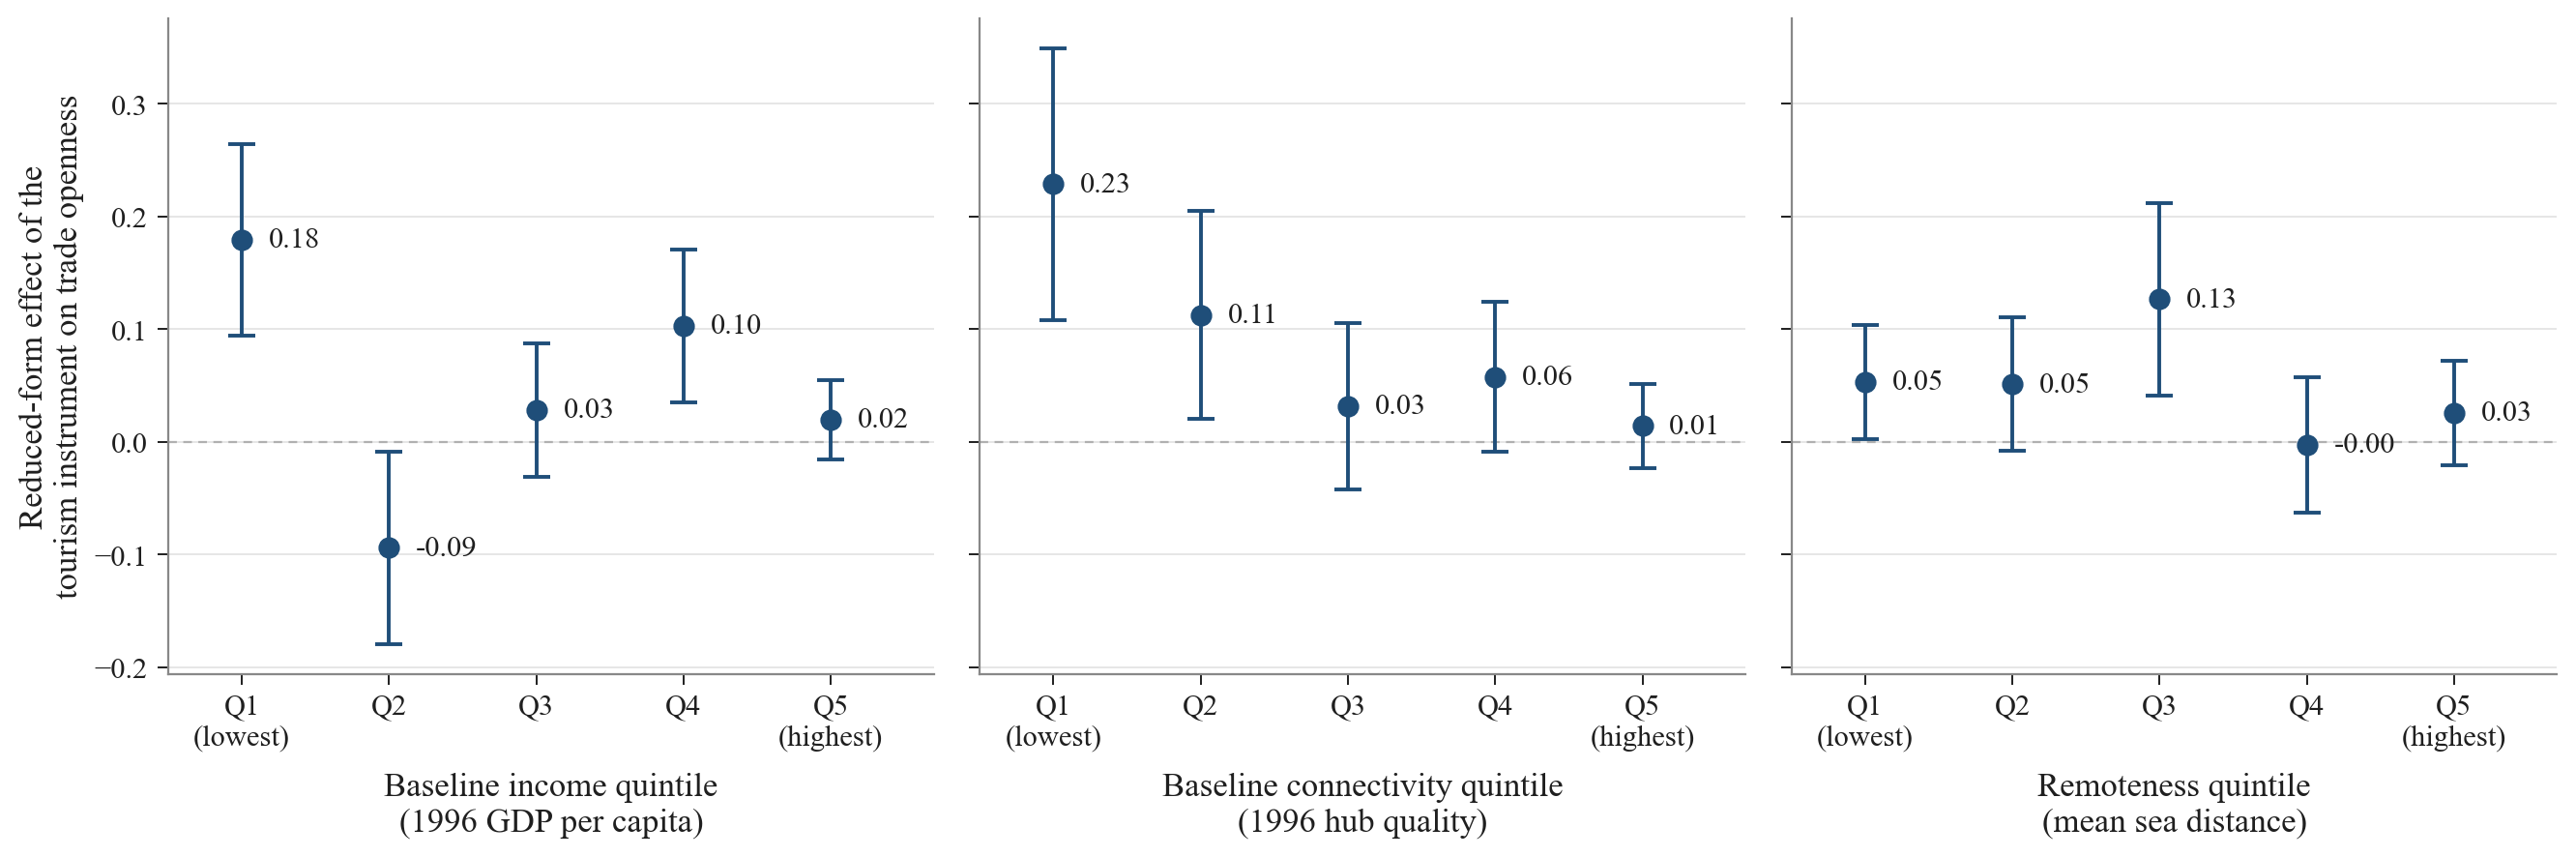
\includegraphics[width=\linewidth]{GACI_rf_quintile.png}
\caption{Flexible reduced-form heterogeneity: effect of the tourism-heritage
instrument on trade openness by quintile bin of baseline income, baseline
connectivity, and remoteness (95\% CIs, robust SE). Bins are country-level
quintiles over the estimation sample; country and year fixed effects absorb
the bin main effects.}
\label{fig:rfquintile}
\end{figure}


\section{Country-level estimates}
\label{app:country}
%=======================================================================
Table~\ref{tab:country} reports, for each country, the implied effect of its
1996--2023 connectivity growth on each outcome and the implied goods-trade gain,
with delta-method standard errors. These are not separately estimated
per-country regressions (a single country's series cannot identify the IV) but
the pooled elasticities applied to each country's observed change in hub
quality; cross-country variation therefore enters only through $\Delta G$.

\begin{table}[H]
\centering
\caption{Country-level implied effects of air-connectivity growth, 1996--2023.}
\label{tab:country}
\begin{threeparttable}
\scriptsize
\begin{tabular}{lrcccr}
\toprule
Country & $\Delta\ln\mathrm{GACI}_{cwm}$ & Openness & Volume & GDP & Trade gain \\
 & & $\beta_{int}\Delta G$ & $\beta_{vol}\Delta G$ & $\beta_{gdp}\Delta G$ & (\$bn) \\
\midrule
\multicolumn{6}{l}{\emph{Largest implied trade gains (top 25)}}\\
CHN & 0.33 & 0.43 (0.22) & 0.76 (0.25) & 0.33 (0.22) & 2062.9 (840.8) \\
KOR & 0.71 & 0.93 (0.47) & 1.64 (0.55) & 0.71 (0.48) & 769.8 (237.8) \\
ARE & 0.57 & 0.74 (0.38) & 1.31 (0.44) & 0.57 (0.39) & 543.9 (186.8) \\
JPN & 0.19 & 0.25 (0.13) & 0.44 (0.15) & 0.19 (0.13) & 330.3 (148.0) \\
TUR & 0.55 & 0.71 (0.36) & 1.26 (0.42) & 0.55 (0.37) & 314.1 (109.6) \\
CAN & 0.22 & 0.29 (0.15) & 0.50 (0.17) & 0.22 (0.15) & 283.2 (124.4) \\
VNM & 0.39 & 0.50 (0.26) & 0.89 (0.30) & 0.39 (0.26) & 268.8 (105.1) \\
SAU & 0.51 & 0.67 (0.34) & 1.18 (0.40) & 0.51 (0.35) & 256.4 (91.7) \\
USA & 0.04 & 0.05 (0.02) & 0.08 (0.03) & 0.04 (0.02) & 242.3 (120.3) \\
IND & 0.19 & 0.24 (0.12) & 0.43 (0.15) & 0.19 (0.13) & 239.3 (107.5) \\
SGP & 0.21 & 0.28 (0.14) & 0.49 (0.16) & 0.21 (0.14) & 216.7 (95.7) \\
POL & 0.21 & 0.27 (0.14) & 0.48 (0.16) & 0.21 (0.14) & 179.9 (79.5) \\
IRL & 0.50 & 0.66 (0.33) & 1.16 (0.39) & 0.50 (0.34) & 173.0 (62.2) \\
MYS & 0.24 & 0.31 (0.16) & 0.55 (0.18) & 0.24 (0.16) & 153.8 (66.7) \\
ESP & 0.14 & 0.18 (0.09) & 0.32 (0.11) & 0.14 (0.09) & 146.0 (67.8) \\
MEX & 0.10 & 0.12 (0.06) & 0.22 (0.07) & 0.10 (0.06) & 141.8 (67.7) \\
NLD & 0.06 & 0.08 (0.04) & 0.14 (0.05) & 0.06 (0.04) & 138.5 (67.6) \\
CZE & 0.24 & 0.31 (0.16) & 0.54 (0.18) & 0.24 (0.16) & 129.0 (56.0) \\
NOR & 0.48 & 0.62 (0.32) & 1.10 (0.37) & 0.48 (0.33) & 128.5 (47.0) \\
HUN & 0.35 & 0.45 (0.23) & 0.80 (0.27) & 0.35 (0.24) & 115.5 (46.4) \\
AUT & 0.21 & 0.28 (0.14) & 0.49 (0.17) & 0.21 (0.15) & 109.6 (48.3) \\
FRA & 0.06 & 0.08 (0.04) & 0.14 (0.05) & 0.06 (0.04) & 107.5 (52.6) \\
QAT & 0.80 & 1.04 (0.53) & 1.85 (0.62) & 0.80 (0.55) & 106.5 (30.7) \\
PRT & 0.39 & 0.51 (0.26) & 0.91 (0.31) & 0.39 (0.27) & 79.0 (30.8) \\
IDN & 0.13 & 0.17 (0.09) & 0.31 (0.10) & 0.13 (0.09) & 76.4 (35.6) \\
\addlinespace
\multicolumn{6}{l}{\emph{Connectivity decliners (bottom 5)}}\\
RUS & -0.01 & -0.02 (0.01) & -0.03 (0.01) & -0.01 (0.01) & -13.5 (6.9) \\
ITA & -0.04 & -0.05 (0.02) & -0.08 (0.03) & -0.04 (0.02) & -63.5 (33.0) \\
UKR & -0.58 & -0.76 (0.39) & -1.34 (0.45) & -0.58 (0.40) & -112.7 (81.7) \\
BEL & -0.10 & -0.13 (0.07) & -0.23 (0.08) & -0.10 (0.07) & -159.2 (86.4) \\
DEU & -0.09 & -0.12 (0.06) & -0.21 (0.07) & -0.09 (0.06) & -406.3 (219.3) \\
\midrule
World total & --- & --- & --- & --- & 7858 \\
\bottomrule
\end{tabular}
\begin{tablenotes}\scriptsize
\item Implied effects apply the pooled cwm IV elasticities (openness
$\beta_{int}=1.302\,(0.662)$, volume $\beta_{vol}=2.303\,(0.776)$, GDP
$\beta_{gdp}=1.001\,(0.680)$) to the change in hub quality
$\Delta\ln\mathrm{GACI}_{cwm}$ observed for each country between its first and
last sample year. Columns 3--5 report the implied log-point effect
$\beta_k\Delta G$ with delta-method SE $\mathrm{SE}(\beta_k)\,|\Delta G|$ in
parentheses. The trade gain is
$\text{goods}\times(1-e^{-\beta_{int}\Delta G})$ with delta-method SE. These are
not separately estimated per-country regressions: cross-country variation enters
only through $\Delta G$. World total is summed over all 184 countries; negative
entries reflect a decline in capacity-weighted hub quality (airspace closures or
capacity re-allocation), not necessarily a fall in total connectivity.
\end{tablenotes}
\end{threeparttable}
\end{table}

\section*{Data and code availability}
GACI is derived from proprietary airline-schedule data; the constructed
country-year panel, instrument inputs (UNESCO, WDI, UNWTO, CERDI, BACI), and
replication scripts are available from the authors on request.

\bibliographystyle{elsarticle-harv}
\bibliography{GACI_TRA_refs}

\end{document}
